% Created 2014-08-19 wto 16:04
\documentclass[a4paper]{article}
\usepackage{fontspec}
\usepackage{fixltx2e}
\usepackage{graphicx}
\usepackage{longtable}
\usepackage{float}
\usepackage{wrapfig}
\usepackage{soul}
\usepackage{textcomp}
\usepackage{marvosym}
\usepackage{wasysym}
\usepackage{latexsym}
\usepackage{amssymb}
\usepackage{hyperref}
\tolerance=1000
\usepackage[margin=2cm]{geometry}
\usepackage{amsmath}
\usepackage{minted}
\usepackage{lscape}
\providecommand{\alert}[1]{\textbf{#1}}

\title{\textbf{Hive v0.1
 - User Guide}}
\author{Kajetan Rzepecki}
\date{\today}

\begin{document}

\maketitle


\vfill
\begin{center}
\includegraphics[scale=1.0]{./img/hive.png}
\end{center}

\vfill

\thispagestyle{empty}
\pagebreak

\tableofcontents

\pagebreak
\section{Dependencies}
\label{sec-1}

The following section lists Hive's dependencies.
\subsection{Erlang/OTP}
\label{sec-1-1}

Hive is known to build and run under \textbf{Erlang R16B} in the following setup:


\begin{verbatim}
$ erl
Erlang R16B (erts-5.10.1) [source-05f1189] [64-bit] [smp:2:2] [async-threads:10]
  [hipe] [kernel-poll:true]
  Eshell V5.10.1
\end{verbatim}



\noindent
Furthermore, Hive uses \textbf{escript} for scripting, so an instance has to be provided (it is usually boundled together with Erlang/OTP).
\subsection{Build tools}
\label{sec-1-2}


\begin{itemize}
\item \textbf{rebar} - Hive uses \href{https://github.com/basho/rebar}{Rebar} build tool for managing library dependencies and the building process in general. A version of \textbf{2.0.0} is required.
\item \textbf{make} - for convenience a \textbf{Makefile} build script is provided that wraps Rebar. Any \textbf{make} will do.
\item \textbf{git} - rebar uses \textbf{git} to fetch library dependencies from GitHub, so \textbf{git} in a recent-ish version is required.
\end{itemize}
\subsection{3rd party libraries}
\label{sec-1-3}

The libraries, listed belowe, are downloaded automatically by Rebar via \textbf{git}, so no special set-up other than \textbf{Rebar and git} is required.


\begin{itemize}
\item \textbf{Lager} - an easy to use logging library found \href{https://github.com/basho/lager}{here}. Hive uses version \textbf{2.0.0}.
\item \textbf{Cowboy} - \href{https://github.com/extend/cowboy}{a web server} optimized for speed. Hive requires Cowboy \textbf{0.8.6}.
\item \textbf{Ranch} - a TCP pool pulled in by Cowboy from \href{https://github.com/extend/ranch}{here}, Hive requires version \textbf{0.8.4}.
\item \textbf{JSONx} - JSON parser optimized for speed, found \href{https://github.com/iskra/jsonx}{here}. There is \textbf{no stable version} as of $\today$; Hive is known to build and run on commit \textbf{a8381a34d126a93eded62c248989dd0529cd257d}, so in case of any problems some fiddling might be required.
\item \textbf{Jesse} - JSON schema validator, found \href{https://github.com/alertlogic/jesse}{here}. Hive is know to build and run using commit \textbf{6bdfce3e988239a8878d7bd19877d7e3d46ae7d7}.
\item \textbf{Ibrowse} - \href{https://github.com/cmullaparthi/ibrowse}{an HTTP client}; Hive uses version \textbf{v4.0.2}.
\end{itemize}

\label{ref-folsom}

\begin{itemize}
\item \textbf{Folsom} - \href{https://github.com/boundary/folsom}{a monitoring tool}; Hive requires version \textbf{0.7.4}.
\item \textbf{Poolboy} - worker pool management library found \href{https://github.com/devinus/poolboy}{here}. Hive requires version \textbf{1.0.0}.
\item \textbf{ERedis} - \href{https://github.com/wooga/eredis}{a Redis connector}, Hive requires version \textbf{v1.0.5}.
\end{itemize}

\pagebreak
\section{Installation \& Running}
\label{sec-2}

The following section describes how to build \& run the Hive server.
\subsection{Obtaining Hive}
\label{sec-2-1}

Use \textbf{git} to clone the repository:


\begin{verbatim}
$ git clone https://host:port/path/to/hive.git hive
\end{verbatim}



\noindent
After the checkout you will be greeted with the following repository layout:


\begin{verbatim}
$ tree hive
  hive
  |-- docs                - Documentation files.
  |   '-- ...
  |-- include             - Erlang header files.
  |   '-- ...
  |-- etc                 - Default configuration files.
  |   |-- schema          - Config validation schema files.
  |   '-- ...
  |-- Makefile            - Build script for make.
  |-- plugins             - Hive plugins directory.
  |   '-- ...
  |-- priv                - Additional scripts directory.
  |   '-- ...
  |-- rebar               - Rebar build tool.
  |-- rebar.config        - Rebar config (lists dependencies).
  |-- src                 - Erlang source files.
  |   '-- ...
  '-- test                - Erlang unit-tests.
      '-- ...
\end{verbatim}
\subsection{Building Hive}
\label{sec-2-2}

Simply type \textbf{make} in the root of the repository and the supplied \textbf{Makefile} script will handle all of the build process for you:


\begin{verbatim}
$ make
\end{verbatim}



\noindent
Building Hive for the first time takes a considerable amount of time as Rebar downloads and compiles all of the dependencies, go grab a coffee! Other build script options:


\begin{itemize}
\item Building a Debian \texttt{.deb} package for easy distribution:
\end{itemize}


\begin{verbatim}
$ make deb-package                                 - Builds using default options.
$ make deb-package TARGET="target --and --options" - Used to pass additional build options.
\end{verbatim}




\begin{itemize}
\item Cleaning up the repository - this will clean up all temporary and compiled files:
\end{itemize}


\begin{verbatim}
$ make clean
\end{verbatim}




\begin{itemize}
\item Unit-testing - this will run \textbf{EUnit} testing framework and dump results into the \textbf{.eunit} directory:
\end{itemize}


\begin{verbatim}
$ make unit-test
\end{verbatim}




\begin{itemize}
\item Testing Hive configuration - this will test the Hive configuration file:
\end{itemize}


\begin{verbatim}
$ make test-config                            - Tests the default configuration file.
$ make test-config CONFIG=path/to/config.json - Tests CONFIG file.
\end{verbatim}




\begin{itemize}
\item Running Hive - this will run Hive as described in the next subsection:
\end{itemize}


\begin{verbatim}
$ make run                                - Runs in production mode.
$ make run CONFIG=path/to/config.json     - Runs in production mode using CONFIG.
$ make run-dev                            - Runs in development mode.
$ make run-dev CONFIG=path/to/config.json - Runs in development mode using CONFIG.
\end{verbatim}
\subsection{Running Hive}
\label{sec-2-3}

Before running Hive make sure that the supplied configuration file is valid and loads properly by invoking:


\begin{verbatim}
$ make test-config CONFIG=path/to/config.json
\end{verbatim}



\noindent
If the configuration file loads properly you can attempt to run Hive. For convenience there's a \textbf{make} rule for that defined in the Makefile:


\begin{verbatim}
$ make run CONFIG=path/to/config.json
\end{verbatim}



\noindent
After a quick boot-up you will be greeted by a log similar to this one (note that the order of the log lines might be different at each execution as Hive consists of multiple processes running in parallel):


\begin{verbatim}
18:21:02.724 [notice] Starting Hive...
18:21:02.734 [notice] Starting Hive Top-level Supervisor...
18:21:02.740 [notice] Starting Hive Environment Supervisor...
18:21:02.769 [notice] Starting Hive Monitor...
18:21:02.780 [notice] Hive Monitor started!
18:21:02.785 [notice] Starting Hive Plugins Manager...
18:21:02.791 [notice] Loading Hive Plugin: plugin_1
...
18:21:02.852 [notice] Hive Plugins Manager started!
18:21:02.860 [notice] Starting Hive Config Manager...
18:21:02.886 [notice] Hive Config Manager started!
18:21:02.887 [notice] Starting Hive Cluster Manager...
18:21:02.887 [notice] Hive Cluster Manager started!
18:21:02.889 [notice] Hive Environment Supervisor started!
18:21:02.894 [notice] Starting Hive Module Supervisor...
18:21:02.918 [notice] Starting Hive Connectors Supervisor...
18:21:02.925 [notice] Starting Hive Connectors Manager...
18:21:02.925 [notice] Hive Connectors Manager started!
18:21:02.926 [notice] Hive Connectors Supervisor started!
18:21:02.932 [notice] Starting Hive Connectors Pool Supervisor...
18:21:02.932 [notice] Hive Connectors Pool Supervisor started!
18:21:02.941 [notice] Starting Hive Router Supervisor...
18:21:02.945 [notice] Starting Hive Connector pool_1...
...
18:21:02.959 [notice] Starting Hive Router...
18:21:02.959 [notice] Hive Router started!
18:21:02.959 [notice] Hive Router Supervisor started!
18:21:02.969 [notice] Starting Hive Clients Supervisor...
18:21:02.969 [notice] Hive Clients Supervisor started!
18:21:02.974 [notice] Starting Hive Pub-Sub Supervisor...
18:21:02.996 [notice] Starting Hive Pub-Sub...
18:21:02.997 [notice] Hive Pub-Sub started!
18:21:02.998 [notice] Hive Pub-Sub Supervisor started!
18:21:03.008 [notice] Starting Hive Pub-Sub Channel Supervisor...
18:21:03.008 [notice] Hive Pub-Sub Channel Supervisor started!
18:21:03.014 [notice] Starting Hive Server Supervisor...
18:21:03.020 [notice] Starting Hive Monitor Server...
18:21:03.041 [notice] Hive Monitor Server started!
18:21:03.046 [notice] Starting Hive API Server...
18:21:03.058 [notice] Hive API Server started!
18:21:03.070 [notice] Starting Hive Server...
18:21:03.085 [notice] Hive Server started!
18:21:03.086 [notice] Hive Server Supervisor started!
18:21:03.086 [notice] Hive Module Supervisor started!
18:21:03.089 [notice] Hive Top-level Supervisor started!
18:21:03.089 [notice] Hive started!
\end{verbatim}



\noindent
\ldots{}and the supervision tree will look something like this:


\begin{verbatim}
hive_root_sup                        - Top-level Hive supervisor.
|-- hive_env_sup                     - Hive environment supervisor.
|   |-- hive_config                  - Hive Config Manager.
|   |-- hive_monitor                 - Hive Monitor Manager.
|   |-- hive_plugins                 - Hive Plugins Manager.
|   '-- hive_cluster                 - Hive Cluster Manager.
'-- hive_sup                         - Hive Modules supervisor.
    |-- hive_connectors_sup          - Hive Connectors supervisor.
    |   |-- hive_connectors          - Hive Connectors Manager.
    |   '-- hive_connectors_pool_sup - Hive Connectors pool supervisor.
    |        |-- connector1          - Various Connectors.
    |        |    '-- ...            - Connector pool workers.
    |        '-- ...
    |-- hive_pubsub_sup              - Pub-Sub supervisor.
    |   |-- hive_pubsub_channel_sup  - Pub-Sub channel supervisor.
    |   |   '-- ...                  - Various Pub-Sub channels.
    |   '-- hive_pubsub              - Pub-Sub manager.
    |-- hive_router_sup              - Router supervisor.
    |   |-- hive_client_sup          - Clients supervisor.
    |   |   '-- ...                  - Client-related processes.
    |   '-- hive_router              - Hive Router.
    '-- hive_web_sup                 - Hive Server & Monitor supervisor.
        |-- hive_api                 - The main Hive API Server entry point.
        |-- hive_monitor_server      - The Hive Monitor Server entry point.
        '-- hive_web                 - The main Hive Server entry point.
\end{verbatim}
\subsection{Stopping Hive}
\label{sec-2-4}

The Hive server employs a \textbf{graceful termination} strategy - after requesting a server termination Clients are asked \emph{nicely} to close their connections and after a certain timeout Hive forces their termination by killing them. No new connections are accepted during the graceful termination period.

\noindent
The configuration parameters responsible for the graceful termination behaviour are described \hyperref[ref-graceful_config]{here}.

\noindent
The graceful termination RESTful API is described \hyperref[sec-6-1-2]{here}.
\subsection{Repository layout reference}
\label{sec-2-5}


\begin{verbatim}
$ tree hive
  hive
  |-- deps                   - Dependencies directory.
  |   '-- ...
  |-- docs                   - Documentation files.
  |   |-- docs.pdf           - YOU ARE HERE.
  |   '-- ...
  |-- ebin                   - Compiled Hive source files.
  |   '-- ...
  |-- etc                    - Hive configuration files.
  |   |-- hive.json          - The default configuration file.
  |   |-- schema             - Hive config validation files.
  |   '-- ...
  |-- include                - Hive Erlang include files.
  |   '-- ...
  |-- log
  |   '-- hive
  |       |-- console.log    - Hive console log (similar to the one in console).
  |       |-- crash.log      - Hive crash log (only crash reports).
  |       '-- error.log      - Hive error log (only error messages).
  |-- Makefile               - Make rules file.
  |-- plugins                - Hive plugins directory (source code).
  |   '-- ...
  |-- priv                   - Directory containing additional stuff.
  |   |-- start-dev.sh       - Hive running script (dev version).
  |   |-- start.sh           - Hive running script.
  |   |-- prep_hive.erl      - A script that prepares Hives execution environment.
  |   |-- test_config.erl    - Hive configuration testing script.
  |   |-- tsung_hive.xml     - A config file for Tsung.
  |   '-- ...
  |-- rebar                  - Rebar build tool.
  |-- rebar.config           - Rebar config (lists dependencies).
  |-- src                    - Hive Erlang source files.
  |   |-- hive_client*       - Hive generic client code.
  |   |-- hive_websocket*    - Hive WebSocket client related code.
  |   |-- hive_xhr_polling*  - Hive XHR-polling client related code.
  |   |---hive_socketio*     - Hive Socket.IO related code.
  |   |-- hive_connectors*   - Hive Connectors manager.
  |   |-- hive_*_connector*  - Various connectors.
  |   |-- hive_*_client*     - Hive Client handler related code.
  |   |-- hive_hooks*        - Hive Hooks related code.
  |   |-- hive_events*       - Hive Internal Events related code.
  |   |-- hive_monitor*      - Hive Monitor related code.
  |   |-- hive_pubsub*       - Hive Pub-Sub related code.
  |   |-- hive_router*       - Hive Router related code.
  |   |-- hive_config*       - Hive Config related code.
  |   |-- hive_cluster*      - Hive Cluster Manager related code.
  |   |-- hive_api*          - Hive RESTful API related code.
  |   |-- hive_*_sup*        - Various Hive supervisors.
  |   '-- ...
  '-- test                   - Hive unit-tests.
      '-- ...
\end{verbatim}



\pagebreak
\section{Configuration \& Tweaking}
\label{sec-3}

The following section lists and describes various configuration parameters and their purpose. The configuration file uses \textbf{JSON} format that is later transformed into Erlang terms. It shouldn't matter, but keep this in mind in case something weird starts to happen \emph{*wink, wink*}. The default configuration file is \textbf{etc/hive.json}.

\noindent
The configuration file is divided into several sections, each of which controls a different part of the Hive server. Section ordering in the configuration file does not matter, neither does parameter ordering mid-section. The general layout of the file is as follows:


\begin{minted}[]{javascript}
{
    "sectionA" : {
        "parameterA" : "valueA",
        "parameterB" : "valueB",
        ...
    },
    "sectionB" : {
        "parameterB" : "valueB",
        "parameterC" : "valueC",
        ...
    },
    ...
}
\end{minted}




\noindent
At the moment, there are several sections recognized by Hive and all of them are required. The sections are:


\begin{minted}[]{javascript}
{
    "hive" : {
        // Contains general Hive related parameters.
    },
    "socketio" : {
        // Contains Socket.IO protocol related parameters.
    },
    "clients" : {
        // Contains Client FSM & Hooks related parameters.
    },
    "connectors" : {
        // Contains parameters controlling various Hive Connectors.
    },
    "pubsub" : {
        // Contains parameters controlling Hive Pub-Sub channels.
    },
    "api" : {
        // Contains parameters controlling the Hive API Server.
    },
    "monitor" : {
        // Contains parameters controlling the Hive Monitor.
    },
    "log" : {
        // Contains logging related parameters.
    }
}
\end{minted}
\subsection{Configuration parameters}
\label{sec-3-1}

Each of the configuration file sections, their parameters (some of which are optional) and accepted values are described in the following subsections. By convention each description will use the full qualified parameter name, for example:


\begin{verbatim}
sectionA.parameterB
sectionB.parameterB
\end{verbatim}
\subsubsection{\texttt{hive}}
\label{sec-3-1-1}

This subsection describes the \textbf{hive} part of the configuration file and corresponds to the general configuration of the Hive server - it contains stuff that didn't really fit elsewhere.

\noindent
Required parameters:

\begin{itemize}
\item \texttt{hive.acceptors} - the number of HTTP acceptors that receive and prepare HTTP connections. It is in no way related to the maximum number of connections. This has to be \textbf{a positive integer}.
\item \texttt{hive.port} - the port on which Hive will listen for incoming connections. It has to be \textbf{a non-negative integer lower than 65536}.
\item \texttt{hive.allowed\_origins} - a JavaScript array of the origins that are allowed to access Hive services. Has to be \textbf{an array of strings}, each of which names a single origin - \textbf{a URL} (possibly with wildcards) or the special value \texttt{null} (equivalent to an undefined origin). Some examples:
\end{itemize}


\begin{minted}[]{javascript}
null, "null", "*.*", "http://zadane.pl"
\end{minted}




\label{ref-graceful_config}

\begin{itemize}
\item \texttt{hive.graceful\_termination\_timeout} - the time (\textbf{in milliseconds}) after which Client Workers will be forced to terminate on server termination.
\item \texttt{hive.max\_client\_slots} - the maximal number of clients that can be connected to Hive. It has to be \textbf{a positive integer}.
\end{itemize}

\noindent
Additional, optional parameters:

\label{ref-cluster-config}

\begin{itemize}
\item \texttt{hive.name} - a string representing the name of this Hive instance, defaults to unqualified ``hive''. It is described in detail in a \hyperref[sec-8-2]{later section}.
\item \texttt{hive.cluster\_name} - a string representing the name of the Hive cluster formed by this Hive instance, defaults to ``hive$_{\mathrm{cluster}}$''.
\item \texttt{hive.cluster\_nodes} - a JavaScript array of node names to which this instance will attept to connect. Every element of this array should be a fully qualified \texttt{hive.name} of another Hive instance.
\item \texttt{hive.cluster\_port\_min} - an integer in range (0, 65535) representing the lower bound of the range of ports used to maintain Hive cluster connections.
\item \texttt{hive.cluster\_port\_max} - an integer in range (0, 65535) representing the upper bound of the range of ports used to maintain Hive cluster connections.
\item \texttt{hive.direct\_websocket} - \textbf{a boolean} flag determining whether WebSocket-based clients should skip the Hive Router in order to speed up the client-server communication. Skipping the router involves a trade off in that the router won't be able to manage clients communication (so no Socket.IO event related router logs, possible message counts inconsistencies, etc).
\item \texttt{hive.websocket\_ping\_timeout} - the timeout (\textbf{in milliseconds}) used by the  WebSocket connection handlers to determine whether they are still active; if there is no pong message received from the client for this amount of time, its Client worker will be terminated. It has to be \textbf{a positive integer}.
\item \texttt{hive.max\_processes} - the maximal number of processes that can exist in the Erlang VM. It has to be \textbf{a positive integer}. Keep in mind that the actual maximal number of processes might be higher (courtesy of the Erlang VM).
\end{itemize}

\noindent
Example values:


\begin{minted}[]{javascript}
"hive" : {
    "name" : "hive@zadane.pl",
    "cluster_name" : "hive_server_cluster",
    "cluster_port_min" : 1234,
    "cluster_port_max" : 2345,

    "acceptors" : 1000,
    "port" : 8080,
    "allowed_origins" : ["http://zadane.pl"],

    "max_client_slots" : 1000,
    "max_processes" : 15000,
    "graceful_termination_timeout" : 10000,

    "direct_websocket" : true,
    "websocket_ping_timeout" : 500
}
\end{minted}
\subsubsection{\texttt{socketio}}
\label{sec-3-1-2}

This subsection describes the \textbf{socketio} part of the configuration file. It is used to tweak the underlying \textbf{Socket.IO protocol}.

\noindent
Required parameters:

\begin{itemize}
\item \texttt{socketio.heartbeat\_timeout} - the heartbeat timeout \textbf{in milliseconds} used by the server (the client receives around 110\% of this value). It has to be \textbf{a positive integer greater than or equal to 1000}.
\item \texttt{socketio.reconnect\_timeout} - the reconnection timeout \textbf{in milliseconds}, currently not used. It has to be \textbf{a positive integer greater than or equal to 1000}.
\item \texttt{socketio.poll\_timeout} - the polling timeout \textbf{in milliseconds}, used by the server to bound message polling times that happens before sending a reply to the client. Has to be \textbf{a positive integer}.
\item \texttt{socketio.init\_timeout} - the initialization timeout \textbf{in milliseconds}, it is started after the Socket.IO handshake in order to make sure that uninitialized clients don't clog the memory for all of eternity and beyond. Again, has to be \textbf{a positive integer}.
\item \texttt{socketio.session\_timeout} - the session timeout \textbf{in milliseconds}; if there are no messages received from the client for this amount of time, its connection will be terminated. It has to be \textbf{a positive integer}.
\item \texttt{socketio.transports} - lists the available transport protocols for use by the Socket.IO protocol. Has to be \textbf{a JavaScript array of strings}, each of which names a single transport. Currently supported transports:
\end{itemize}


\begin{minted}[]{javascript}
"xhr-polling", "websocket", "flashsocket"
\end{minted}




\noindent
Example values:


\begin{minted}[]{javascript}
"socketio" : {
    "heartbeat_timeout" : 30000,
    "reconnect_timeout" : 120000,
    "poll_timeout" : 500,
    "init_timeout" : 5000,
    "session_timeout" : 120000,
    "transports" : ["websocket", "xhr-polling"]
}
\end{minted}
\subsubsection{\texttt{clients}}
\label{sec-3-1-3}

This subsection describes the \textbf{clients} part of the configuration file and corresponds to the general configuration of the Hive Client FSMs.

\noindent
Required parameters:


\begin{itemize}
\item \texttt{clients.state} - the descriptor of a State Manager to be used by the Client processes. It has to be \textbf{a JSON object} containing exactly three fields: \texttt{state\_manager}, \texttt{initial\_value} and \texttt{args}. State Management and available State Managers are described in greater detail in \hyperref[sec-7-1-5]{a later section}.
\end{itemize}

\label{ref-events_config}

\begin{itemize}
\item \texttt{clients.actions} - \textbf{a JSON object} listing various \textbf{internal event} dispatchers recognized by the Client Workers on a \textbf{per-action} basis, that is, each field names an action will trigger Hive Internal Event dispatchers listed in this field's value. The value has to be \textbf{a JavaScript array} of Hive Internal Event dispatcher descriptors, each of which has to be \textbf{a JSON object} that defines several fields:
\begin{itemize}
\item \texttt{action} - the name of the Hive Internal Event dispatcher to run when triggered. Available Hive Internal Event dispatchers are described in greated detail in \hyperref[sec-9-3]{a later section}.
\item \texttt{args} - the arguments passed to the Hive Internal Event dispatcher when it is run. Accepted argument descriptions are found in \hyperref[sec-9-3]{a later section}.
\end{itemize}
\end{itemize}

\label{ref-hooks_config}

\begin{itemize}
\item \texttt{clients.hooks} - \textbf{a JSON object} containing various Hive Hook definitions on a \textbf{per-event} basis, that is, each field of the JSON object names an event that will trigger Hive Hooks listed in this field's value. The value has to be \textbf{a JavaScript array} of Hive Hook descriptors, each of which has to be \textbf{a JSON object} that defines several fields:
\begin{itemize}
\item \texttt{hook} - the name of the Hive Hook to run when triggered. Available Hive Hooks are described in greated detail in \hyperref[sec-9-2]{a later section}.
\item \texttt{args} - the arguments passed to the Hive Hook when it is run. Accepted arguments descriptions are found in \hyperref[sec-9-2]{a later section}.
\end{itemize}
\end{itemize}

\noindent
Example values:


\begin{minted}[]{javascript}
"clients" : {
    "state" : {
        "state_manager" : "sm.redis",
        "initial_value" : [1, 2, 3],
        "args" : {
            "connector" : "database",
            "expiration_timeout" : 60000
        }
    },
    "actions" : {
        "action_1" : [
            {
                "action" : "action.store",
                "args" : null
            },
            ...
        ],
        ...
    },
    "hooks" : {
        "event_1" : [
            {
                "hook" : "utils.echo",
                "args" : null
            },
            ...
        ],
        ...
    }
}
\end{minted}
\subsubsection{\texttt{connectors}}
\label{sec-3-1-4}

This subsection describes the \textbf{connectors} part of the configuration file. It is used to control various Hive Connectors.

\noindent
Required parameters:

\begin{itemize}
\item \texttt{connectors.rent\_timeout} - the timeout \textbf{in milliseconds} used when waiting for an available worker in a given connectors pool. If there are no available workers in a pool, the renting process will wait for at most this much time. It has to be \textbf{a positive integer}.
\end{itemize}

\label{ref-connectors_config}

\begin{itemize}
\item \texttt{connectors.pools} - \textbf{a JSON object} of \textbf{name/pool descriptor} pairs - pairs of \textbf{strings} representing pool names and \textbf{JSON objects} representing pools themselves. Each pool descriptor has to define several required parameters:
\begin{itemize}
\item \texttt{size} - the base size of the pool; \textbf{a non-negative integer}.
\item \texttt{overflow} - the maximum number of additional workers that are created under heavy server load (the total number of available workers is therefore \texttt{size} + \texttt{overflow}). It has to be \textbf{a non-negative integer}.
\item \texttt{args} - the arguments that will be passed to the connector workers at initialization. The accepted values depend heavily on the type of the connector, and will be described later in \hyperref[sec-9-4]{an appropriate section}.
\item \texttt{connector} - the name of the connector plugin to use for this pool. It has to be \textbf{a string}. The available Connector pools will be described in \hyperref[sec-9-4]{a later section}.
\end{itemize}
\end{itemize}

\noindent
Example values:


\begin{minted}[]{javascript}
"connectors" : {
    "rent_timeout" : 5000,
    "pools" : {
        "database" : {
            "connector" : "connector.redis",
            "size" : 100,
            "overflow" : 50,
            "args": {
                "host" : "127.0.0.1",
                "port" : 6379,
                "database" : 0,
                "password" : "",
                "reconnect_timeout" : 100
            }
        }
    }
}
\end{minted}
\subsubsection{\texttt{pubsub}}
\label{sec-3-1-5}

This subsection describes the \textbf{pubsub} portion of the configuration file. It is used to control the Hive Pub-Sub facitily. More about the Hive Pub-Sub can be found in \hyperref[sec-7-3]{a later section}.

\noindent
Required parameters:

\label{ref-pubsub_config}

\begin{itemize}
\item \texttt{pubsub.channels} - \textbf{a JSON object} containing various Hive Pub-Sub channel definitions on \textbf{a per-prefix} basis, that is, each field of the JSON object names a Pub-Sub channel prefix which might later generate concrete Pub-Sub channels. Each \textbf{channel descriptor} has to be \textbf{a JSON object} that defines several fields:
\begin{itemize}
\item \texttt{timeout} - the time (\textbf{in milliseconds}) after which the channel will cease to exist if there are no more Client workers subscribed to it. It has to be \textbf{a non-negative integer}. A timeout of \textbf{0 means infinity (obviously)} - a permanent channel that never ceases to exist.
\item \texttt{privilege} - the access type of a channel, specifies the privilege level required to operate (subscribe or unsubscribe) on a channel. It has to be \textbf{a string}. Accepted values:
\end{itemize}
\end{itemize}


\begin{minted}[]{javascript}
"private", "public"
\end{minted}




\noindent
Example values:


\begin{minted}[]{javascript}
"pubsub" : {
    "channels" : {
        "foo" : {
            "privilege" : "public",
            "timeout" : 1000
        },

        "bar" : {
            "privilege" : "private",
            "timeout" : 0
        }
    }
}
\end{minted}
\subsubsection{\texttt{api}}
\label{sec-3-1-6}
\label{ref-api_config}

This subsection describes the \textbf{api} part of the configuration file. Parameters described in this section control the behaviour of the Hive API Server.

\noindent
Required parameters:

\begin{itemize}
\item \texttt{api.acceptors} - similar to \texttt{server.acceptors}, names the number of HTTP listeners that accept new HTTP connections. Has to be \textbf{a positive integer}.
\item \texttt{api.port} - the port used by the API Server to listen for HTTP connections. Has to be \textbf{a non-negative integer that is lower than 65536}.
\item \texttt{api.hash} - an API key used to secure the Hive API Server accesses. It has to be \textbf{a string of length 8 or more}.
\end{itemize}

\noindent
Example values:

\begin{minted}[]{javascript}
"api" : {
    "acceptors" : 100,
    "port" : 1235,
    "hash" : "abcde12345"
}
\end{minted}
\subsubsection{\texttt{monitor}}
\label{sec-3-1-7}
\label{ref-monitor_config}

This subsection describes the \textbf{monitor} part of the configuration file. It controls the behaviour of the Hive Monitor.

\noindent
Required parameters:

\begin{itemize}
\item \texttt{monitor.acceptors} - similarily to \texttt{server.acceptors} names the number of HTTP listeners that accept new HTTP connections. Has to be \textbf{a positive integer}.
\item \texttt{monitor.port} - the port used by the Monitor to listen for HTTP connections. Has to be \textbf{a non-negative integer that is lower than 65536}.
\item \texttt{monitor.hash} - an API key used to secure the Hive Monitor accesses. It has to be \textbf{a string of length 8 or more}.
\end{itemize}

\noindent
Example values:


\begin{minted}[]{javascript}
"monitor" : {
    "acceptors" : 100,
    "port" : 1234,
    "hash" : "12345abcde"
}
\end{minted}
\subsubsection{\texttt{log}}
\label{sec-3-1-8}
\label{ref-log-config}

This subsection describes the \textbf{log} part of the configuration file. It controls the behaviour of the logger.

\noindent
Required parameters:

\begin{itemize}
\item \texttt{log.dir} - the directory name for log files and crash dumps to reside on the hard drive. Has to be \textbf{a string naming a valid file system location} (the directory does not have to exist).
\end{itemize}

\noindent
Additional, optional parameters:

\begin{itemize}
\item \texttt{log.file\_level} - the minimal log-level of messages dumped to the \texttt{log.file} (``none'' turns off any file logging). Has to be any of the following:
\end{itemize}


\begin{minted}[]{javascript}
"debug", "info", "notice", "warning", "error", "critical", "alert", "emergency", "none"

// Additional filter specifies:
"info"     // Info and higher (>= is implicit).
"=debug"   // Only the debug level.
"!=info"   // Everything but the info level.
"<=notice" // Notice and below.
"<warning" // Anything less than warning.
\end{minted}





\begin{itemize}
\item \texttt{log.console\_level} - the minimal log-level of messages dumped to the console (``none'' turns off any console logging). Has to be any of the following:
\end{itemize}


\begin{minted}[]{javascript}
"debug", "info", "notice", "warning", "error", "critical", "alert", "emergency" "none"

// Additional filter specifies:
"info"     // Info and higher (>= is implicit).
"=debug"   // Only the debug level.
"!=info"   // Everything but the info level.
"<=notice" // Notice and below.
"<warning" // Anything less than warning.
\end{minted}




\noindent
Example values:


\begin{minted}[]{javascript}
"log" : {
    "dir" : "log/",
    "console_level" : "debug",
    "file_level" : "info"
}
\end{minted}
\subsection{Configuration validation}
\label{sec-3-2}

The configuration file can be validated using a supplied configuration testing script by invoking the following command in the root directory of the repository:


\begin{verbatim}
$ make testconfig CONFIG=path/to/config.json
\end{verbatim}



\noindent
Hive uses \textbf{JSON Schema} to validate its configuration files. The schema files used by the Hive Config validator can be found in \textbf{etc/schema} directory in the root repository. Each configuration sections' schema resides in a separate file named \textbf{section.jsonschema}. When defining new configuration parameters it is essential to include them in the validation schema.
\subsection{Organizing the configuration}
\label{sec-3-3}

For convenience each configuration section can be stored in its own, separate file. If that is the case, the main configuration file has to list the file-name where a section configuration can be found relative to the main config file. For example:


\begin{minted}[]{javascript}
{
    "hive" : {
        // Some setup...
    },

    "socketio" : "path/to/socketio.json",

    "clients" : "path/to/clients.json",

    "connectors" : {
        // Some setup...
    },
    ...
}
\end{minted}




\pagebreak
\section{Monitoring \& Statistics}
\label{sec-4}

This section describes the monitoring facilities of the Hive server. Statistics gathering is performed by changing values of various in-memory counters during Hive run-time, using \hyperref[ref-folsom]{Folsom} external library. Most of the counters are represented by \textbf{non-negative integers}, and each of them corresponds to a specific metric of the Hive server.
\subsection{Statistics structure}
\label{sec-4-1}
\label{ref-statistics-structure}


There are many different metrics which are grouped into several sections, and subsections. The structure of the statistics sections is shown below:


\begin{minted}[]{javascript}
{
    "hive" : {
        // Various general metrics.
        "memory" : {
            // Memory usage related metrics.
        },
        "router" : {
            // Hive Router related metrics.
        },
        "cluster" : {
            // Hive Cluster related metrics.
        }
    },
    "clients" : {
        // Various general, client related metrics.
        "state_mgr" : {
            // Client State Manager related metrics.
        },
        "states" : {
            // Client FSM state related metrics.
        },
        "events" : {
            // Dispatched Socket.IO/internal events related metrics.
        },
        "transports" : {
            // Socket.IO transports related metrics.
        },
        "hooks" : {
            // Hive Hooks related metrics.
            "event1" : {
                // Hive Hooks related metrics (per event name).
            },
            ...
        }
    },
    "connectors" : {
        // Various Hive Connectors related metrics.
        "http" : {
            "connector1" : {
                // HTTP Connectors related metrics (per pool name).
            },
            ...
        },
        "redis" : {
            // Redis Connectors related metrics (per pool name).
            ...
        },
        "tcp" : {
            // TCP Connectors related metrics (per pool name).
            ...
        },
        ...
    },
    "pubsub" : {
        // Hive Pub-Sub related metrics.
        "channel_prefix1" : {
            // Various channel prefix related metrics.
        },
        ...
    },
    "api" : {
        // Hive API Server related metrics.
    },
    ...
}
\end{minted}
\subsection{Statistics metrics}
\label{sec-4-2}

Each section and its metrics are described in the following subsections. By convention each description will use the full qualified metric name, for example:


\begin{verbatim}
hive.memory.total
connectors.redis.pool_name_2.errors
\end{verbatim}
\subsubsection{\texttt{hive}}
\label{sec-4-2-1}

This subsection describes the \textbf{hive} portion of the Hive statistics. Metrics found in this subsection measure various general quantities that didn't fit elsewhere:


\begin{itemize}
\item \texttt{hive.uptime} - the uptime (\textbf{in milliseconds}) of the Hive.
\item \texttt{hive.errors} - the number of \textbf{critical} (mostly supervision tree related) Hive errors encountered; it \textbf{does not} include errors from other sections.
\item \texttt{hive.total\_processes} - the number of Erlang processes currently executing in the VM.
\item \texttt{hive.plugins} - the number of currently loaded Hive Plugins.
\item \texttt{hive.plugin\_errors} the number of Hive Plugin related errors.
\item \texttt{hive.config\_errors} the number of Hive Manager errors.
\end{itemize}
\subsubsection{\texttt{hive.memory}}
\label{sec-4-2-2}

This subsection describes the \textbf{hive.memory} portion of the Hive statistics. Metrics found in this subsection measure the memory usage of the Hive Server:


\begin{itemize}
\item \texttt{hive.memory.total} - the total amount of memory used by the Erlang VM.
\item \texttt{hive.memory.processes} - the amount of memory used by the Erlang processes.
\item \texttt{hive.memory.system} - the amount of memory not directly related to any Erlang process. It includes \texttt{atom}, \texttt{binary}, \texttt{code} and \texttt{ets} values.
\item \texttt{hive.memory.atom} - the amount of memory used by the Erlang Atom table. This metric \textbf{does not decrease} as Atoms are not garbage collected by the Erlang VM.
\item \texttt{hive.memory.binary} - the amount of memory used by the Erlang VM to share binary data between the processes.
\item \texttt{hive.memory.code} - the amount of memory used by the loaded Erlang code.
\item \texttt{hive.memory.ets} - the amount of memory used by the Erlang ETS tables.
\end{itemize}
\subsubsection{\texttt{hive.router}}
\label{sec-4-2-3}

This subsection describes the \textbf{hive.router} portion of the Hive statistics. Metrics found in this subsection measure the state of the Hive Router:


\begin{itemize}
\item \texttt{hive.router.uptime} - the router uptime (\textbf{in milliseconds}).
\item \texttt{hive.router.spawned\_clients} - the total number of client processes ever spawned by the Router.
\item \texttt{hive.router.current\_clients} - the current number of running client processes managed by the Router.
\item \texttt{hive.router.requests} - the total number of requests processed by the Router.
\item \texttt{hive.router.msg\_queue\_length} - the length of the Erlang message queue of the Router process. Corresponds directly to the number of requests queued on the router.
\item \texttt{hive.router.routed\_events} - the total number of internal events routed to the client processes by the Router.
\item \texttt{hive.router.routed\_msgs} - the total number of Socket.IO messages (external events) routed to the client processes by the Router.
\item \texttt{hive.router.errors} - the total number of failed requests and other errors encountered by the Router.
\end{itemize}
\subsubsection{\texttt{hive.cluster}}
\label{sec-4-2-4}

This subsection describes the \textbf{hive.cluster} portion of the Hive statistics. Metrics found in this subsection measure the state of the Hive Cluster Manager of a node:


\begin{itemize}
\item \texttt{hive.cluster.nodes} - a JavaScript array of strings listing other connected Hive nodes,
\item \texttt{hive.cluster.size} - the number of nodes currently connected to the cluster,
\item \texttt{hive.cluster.calls} - the total number of cluster wide, synchronous requests performed by this nodes Cluster Manager,
\item \texttt{hive.cluster.casts} - the total number of cluster wide, asynchronous requests performed by this nodes Cluster Manager,
\item \texttt{hive.cluster.errors} - the total number of failed requests and other errors encountered by the Cluster Manager.
\end{itemize}
\subsubsection{\texttt{clients}}
\label{sec-4-2-5}

This subsection describes the \textbf{clients} part of the Hive statistics. Each metric found in this section measures the general quantities related to the Client FSMs:


\begin{itemize}
\item \texttt{clients.total} - the total number of alive clients (for Router debugging purposes).
\item \texttt{clients.websocket} - the total number of alive WebSocket-based clients.
\item \texttt{clients.xhr\_polling} - the total number of alive XHR-polling-based clients.
\item \texttt{clients.errors} - the total number of errors encountered by the client processes.
\end{itemize}
\subsubsection{\texttt{clients.states}}
\label{sec-4-2-6}

This subsection describes the \textbf{clients.states} portion of the Hive statistics. Each metric found here describes the operation of the Client FSMs - state transitions and such:


\begin{itemize}
\item \texttt{clients.states.generic} - the total number of generic (uninitialized via Socket.IO handshake) clients.
\item \texttt{clients.states.transient} - the total number of clients in \textbf{transient} state - clients that are unable to send Socket.IO messages for various reasons (for example, waiting for XHR-polling GET request).
\item \texttt{clients.states.waiting} - the total number of clients in \textbf{waiting} state - clients ready to communicate, but awaiting a response/action from the Hive server.
\item \texttt{clients.states.polling} - the total number of clients in \textbf{polling} state - clients buffering and processing replies.
\item \texttt{clients.states.transitions} - the total number of state transitions of the client FSMs.
\end{itemize}
\subsubsection{\texttt{clients.events}}
\label{sec-4-2-7}

This subsection describes the \textbf{clients.events} portion of the Hive statistics. Each metric found here describes the the operation of the Client logic - dispatched Socket.IO events, events received from the rest of the Hive server, etc:


\begin{itemize}
\item \texttt{clients.events.total} - the total number of events processed by the Client processes, includes \texttt{control}, \texttt{external} and \texttt{internal}.
\item \texttt{clients.events.errors} - the total number of event related errors encountered by the Client processes, includes \texttt{control\_errors}, \texttt{external\_errors} and \texttt{internal\_errors}.
\item \texttt{clients.events.external} - the total number of external events (Socket.IO messages received) processed by the Client processes.
\item \texttt{clients.events.internal} - the total number of internal events (internal messages and Socket.IO replies) processed by the Client processes.
\item \texttt{clients.events.control} - the total number of control events (messages used internally by various Hive submodules) processed by the Client processes.
\item \texttt{clients.events.internal\_errors} - the total number of errors encountered when processing internal events.
\item \texttt{clients.events.external\_errors} - the total number of errors encountered when processing external events (Socket.IO messages).
\item \texttt{clients.events.control\_errors} - the total number of errors encountered when processing control events.
\end{itemize}
\subsubsection{\texttt{clients.state\_mgr}}
\label{sec-4-2-8}

This subsection describes the \textbf{clients.state\_mgr} portion of the Hive statistics. Metrics in this subsection correspond to various Client State Manager quantities.


\begin{itemize}
\item \texttt{clients.state\_mgr.requests} - the total number of State Manager requests.
\item \texttt{clients.state\_mgr.errors} - the total number of errors encountered by the State Manager.
\item \texttt{clients.state\_mgr.init} - the total number of State Manager \texttt{init} requests.
\item \texttt{clients.state\_mgr.get} - the total number of State Manager \texttt{get} requests.
\item \texttt{clients.state\_mgr.set} - the total number of State Manager \texttt{set} requests.
\item \texttt{clients.state\_mgr.cleanup} - the total number of State Manager \texttt{cleanup} requests.
\end{itemize}
\subsubsection{\texttt{clients.transports}}
\label{sec-4-2-9}

This subsection describes the \textbf{clients.transports} portion of the Hive statistics. Metrics in this subsection measure the underlying transport protocols state and operation. Currently there are two subsections defined, for \textbf{WebSocket} and \textbf{XHR-polling} transports respectively:


\begin{itemize}
\item \texttt{clients.transports.http.requests} - the total number of HTTP requests received (includes the Socket.IO handshakes but not HTTP Connectors, etc).
\item \texttt{clients.transports.http.errors} - the total number of bad requests and errors encountered by the transports.
\item \texttt{clients.transports.http.2XX} - the total number of HTTP code 2XX replies.
\item \texttt{clients.transports.http.4XX} - the total number of HTTP code 4XX replies.
\item \texttt{clients.transports.http.5XX} - the total number of HTTP code 5XX replies.
\item \texttt{clients.transports.http.???} - the total number of HTTP replies with other codes.
\item \texttt{clients.transports.http.hang\_up} - the total number of prematurely closed connections (for example, browser closing).
\item \texttt{clients.transports.websocket.requests} - the total number of WebSocket requests (corresponds directly to the number of WebSocket protocol upgrades).
\item \texttt{clients.transports.websocket.errors} - the total number of errors encountered when processing WebSocket errors.
\item \texttt{clients.transports.websocket.frames} - the total number of WebSocket frames received.
\item \texttt{clients.transports.websocket.ok} - the total number of ``good'' WebSocket replies (analogous to \texttt{http.2XX}).
\item \texttt{clients.transports.websocket.bad} - the total number of ``bad'' WebSocket replies (analogous to \texttt{http.4XX} and \texttt{http.5XX}).
\item \texttt{clients.transports.websocket.hang\_up} - the total number of prematurely closed connections (for example, browser closing).
\end{itemize}
\subsubsection{\texttt{clients.hooks}}
\label{sec-4-2-10}

This subsection describes the \textbf{clients.hooks} portion of the Hive statistics. Metrics in this subsection measure various quantities related to the Hive Hooks facility:


\begin{itemize}
\item \texttt{clients.hooks.calls} - the total number of Hive Hooks invocations (either due to Client Messages or external dispatch requests).
\item \texttt{clients.hooks.errors} - the total number of Hive Hooks errors encountered by the Client processes.
\end{itemize}

\noindent
Additionally, the same set of counters is defined on a per-hook-event basis. For an event named \textbf{\$(name)}, the folowing counters will be added to the Monitor. Due to the dynamic nature of the hooks and their per-client character, \textbf{counters described below are added on use} and may not be included in the Monitor output at all times:


\begin{itemize}
\item \texttt{clients.hooks.\$(name).calls} - the total number of Hive Hooks invocations.
\item \texttt{clients.hooks.\$(name).errors} - the total number of Hive Hooks errors encountered by the Client processes.
\end{itemize}
\begin{itemize}

\item \texttt{clients.hooks.hp}\\
\label{sec-4-2-10-1}%
The Hive Protocol hook related metrics.


\begin{itemize}
\item \texttt{clients.hooks.hp.get} - the total number of \texttt{hp.get} Hook invocations.
\item \texttt{clients.hooks.hp.put} - the total number of \texttt{hp.put} Hook invocations.
\item \texttt{clients.hooks.hp.post} - the total number of \texttt{hp.post} Hook invocations.
\end{itemize}

\noindent
Additionally, the same set of counters is defined on a per-hook-event basis. For an event named \textbf{\$(name)}, the folowing counters will be added to the Monitor. Due to the dynamic nature of the hooks and their per-client character, \textbf{counters described below are added on use} and may not be included in the Monitor output at all times:


\begin{itemize}
\item \texttt{clients.hooks.\$(name).hp.get} - the total number of \texttt{hp.get} Hook invocations.
\item \texttt{clients.hooks.\$(name).hp.put} - the total number of \texttt{hp.put} Hook invocations.
\item \texttt{clients.hooks.\$(name).hp.post} - the total number of \texttt{hp.post} Hook invocations.
\end{itemize}


\item \texttt{clients.hooks.pubsub}\\
\label{sec-4-2-10-2}%
The Hive Pub-Sub hook related metrics.


\begin{itemize}
\item \texttt{clients.hooks.pubsub.publish} - the total number of Pub-Sub channel publish requests.
\item \texttt{clients.hooks.pubsub.subscribe} - the total number of Pub-Sub channel subscriptions.
\item \texttt{clients.hooks.pubsub.unsubscribe} - the total number of Pub-Sub channel unsubscriptions.
\end{itemize}

\noindent
Additionally, the same set of counters is defined on a per-hook-event basis. For an event named \textbf{\$(name)}, the folowing counters will be added to the Monitor. Due to the dynamic nature of the hooks and their per-client character, \textbf{counters described below are added on use} and may not be included in the Monitor output at all times:


\begin{itemize}
\item \texttt{clients.hooks.\$(name).pubsub.publish} - the total number of \textbf{name} channel publish requests.
\item \texttt{clients.hooks.\$(name).pubsub.subscribe} - the total number of \textbf{name} channel subscriptions.
\item \texttt{clients.hooks.\$(name).pubsub.unsubscribe} - the total number of \textbf{name} channel unsubscriptions.
\end{itemize}

\end{itemize} % ends low level
\subsubsection{\texttt{connectors}}
\label{sec-4-2-11}

This subsection describes the \textbf{connectors} part of the Hive statistics. Each metric found here measures the general quantities related to the Hive Connectors:


\begin{itemize}
\item \texttt{connectors.requests} - the total number of requests to the Connectors Manager.
\item \texttt{connectors.errors} - the total number of errors encountered by the Connectors Manager.
\item \texttt{connectors.pools} - the total number of connector pools running in the Hive server.
\item \texttt{connectors.starts} - the total number of pool starts.
\item \texttt{connectors.stops} - the total number of pool stops.
\item \texttt{connectors.unsafe\_transactions} - the total number of unsafe transactions performed on the Connector pools.
\item \texttt{connectors.safe\_transactions} - the total number of safe transactions performed on the Connector pools.
\item \texttt{connectors.rents} - the total number of Connector rents (acquisition from a pool for later use).
\item \texttt{connectors.returns} - the total number of Connector returns (returns to a pool).
\end{itemize}

\noindent
The connector pools are grouped by their type and the name they were given, so it is possible to measure multiple instances of each connector pool type.
\subsubsection{\texttt{connectors.http}}
\label{sec-4-2-12}

This subsection describes the \textbf{connectors.http.\$(name)} portion of the Hive statistics. Each metric found here is related to an HTTP connector pool named \textbf{name}:


\begin{itemize}
\item \texttt{connectors.http.\$(name).workers} - the total number of active workers in the pool.
\item \texttt{connectors.http.\$(name).requests} - the total number of requested actions performed by the workers.
\item \texttt{connectors.http.\$(name).errors} - the total number of errors encountered by the workers.
\item \texttt{connectors.http.\$(name).sync\_gets} - the total number of synchronous GET requests requested.
\item \texttt{connectors.http.\$(name).sync\_posts} - the total number of synchronous POST requests.
\item \texttt{connectors.http.\$(name).async\_posts} - the total number of asynchronous POST requests.
\end{itemize}
\subsubsection{\texttt{connectors.redis}}
\label{sec-4-2-13}

This subsection describes the \textbf{connectors.redis.\$(name)} portion of the Hive statistics. Each metric in this subsection is related to the Redis connector pool named \textbf{name}:


\begin{itemize}
\item \texttt{connectors.redis.\$(name).workers} - the total number of active workers in the pool.
\item \texttt{connectors.redis.\$(name).requests} - the total number of requested actions performed by the workers.
\item \texttt{connectors.redis.\$(name).errors} - the total number of errors encountered by the workers.
\item \texttt{connectors.redis.\$(name).queries} - the total number of Redis queries sent by the workers.
\end{itemize}
\subsubsection{\texttt{connectors.tcp}}
\label{sec-4-2-14}

This subsection describes the \textbf{connectors.tcp.\$(name)} part of the Hive statistics. Each metric in here is related to the TCP connector pool named \textbf{name}:


\begin{itemize}
\item \texttt{connectors.tcp.\$(name).workers} - the total number of active workers in the pool.
\item \texttt{connectors.tcp.\$(name).requests} - the total number of requested actions performed by the workers.
\item \texttt{connectors.tcp.\$(name).errors} - the total number of errors encountered by the workers.
\item \texttt{connectors.tcp.\$(name).send} - the total number of \textbf{send} requests processed by the workers.
\item \texttt{connectors.tcp.\$(name).recv} - the total number of \textbf{recv} requests processed by the workers.
\end{itemize}
\subsubsection{\texttt{pubsub}}
\label{sec-4-2-15}

This subsection describes the \textbf{pubsub} portion of the Hive statistics. Metrics in this subsection measure various quantities related to the Hive Pub-Sub facility:


\begin{itemize}
\item \texttt{pubsub.uptime} - the uptime (in \textbf{milliseconds}) of the Hive Pub-Sub Manager.
\item \texttt{pubsub.requests} - the total number of Hive Pub-Sub requests.
\item \texttt{pubsub.errors} - the total number of errors encountered by Hive Pub-Sub facility.
\item \texttt{pubsub.total\_channels} - the total number of active Hive Pub-Sub channels.
\item \texttt{pubsub.status} - the total number of \texttt{status} requests issued to the Pub-Sub channels.
\item \texttt{pubsub.subscribe} - the total number of \texttt{subscribe} requests issued to the Pub-Sub channels.
\item \texttt{pubsub.unsubscribe} - the total number of \texttt{unsubscribe} requests issued to the Pub-Sub channels.
\item \texttt{pubsub.join} - the total number of \texttt{join} requests issued to the Pub-Sub channels.
\item \texttt{pubsub.leave} - the total number of \texttt{leave} requests issued to the Pub-Sub channels.
\item \texttt{pubsub.publish} - the total number of \texttt{publish} requests issued to the Pub-Sub channels.
\item \texttt{pubsub.published\_events} - the total number of events published on the Pub-Sub channels.
\end{itemize}

\noindent
Additionally, a similar set of counters is defined on a per-channel-prefix basis. For a channel prefixed \textbf{\$(name)}, the folowing counters will be added to the Monitor.


\begin{itemize}
\item \texttt{pubsub.channels.\$(name).requests} - the total number of Hive Pub-Sub requests issued to channels with prefix \textbf{name}.
\item \texttt{pubsub.channels.\$(name).errors} - the total number of errors encountered by Hive Pub-Sub channels with prefix \textbf{name}.
\item \texttt{pubsub.channels.\$(name).total\_channels} - the total number of active Hive Pub-Sub channels with prefix \textbf{name}.
\item \texttt{pubsub.channels.\$(name).status} - the total number of \texttt{status} requests issued to channels with prefix \textbf{name}.
\item \texttt{pubsub.channels.\$(name).subscribe} - the total number of \texttt{subscribe} requests issued to channels with prefix \textbf{name}.
\item \texttt{pubsub.channels.\$(name).unsubscribe} - the total number of \texttt{unsubscribe} requests issued to channels with prefix \textbf{name}.
\item \texttt{pubsub.channels.\$(name).publish} - the total number of \texttt{publish} requests issued to channels with prefix \textbf{name}.
\item \texttt{pubsub.channels.\$(name).subscribed\_clients} - the total number of Clients subscribed to channels with prefix \textbf{name} (note that a Client subscribed to several channels with the same prefix \textbf{will appear multiple times in this metric}).
\item \texttt{pubsub.channels.\$(name).published\_events} - the total number of events published on channels with prefix \textbf{name}.
\end{itemize}
\subsubsection{\texttt{api}}
\label{sec-4-2-16}

This subsection describes the \textbf{api} portion of the Hive statistics. Metrics in this subsection measure various quantities related to the Hive API Server:


\begin{itemize}
\item \texttt{api.requests} - the total number of Hive API Server requests.
\item \texttt{api.errors} - the total number of errors encountered by the Hive API Server while processing requests.
\end{itemize}
\subsubsection{\texttt{api.hive}}
\label{sec-4-2-17}

This subsection describes the \textbf{api.hive} portion of the Hive statistics. Metrics in this subsection measure various quantities related to the Pub-Sub part of the Hive API:


\begin{itemize}
\item \texttt{api.hive.requests} - the total number of Hive API Server related requests.
\item \texttt{api.hive.errors} - the total number of errors encountered by the Hive API Server while processing general requests.
\end{itemize}
\subsubsection{\texttt{api.router}}
\label{sec-4-2-18}

This subsection describes the \textbf{api.router} portion of the Hive statistics. Metrics in this subsection measure various quantities related to the Pub-Sub part of the Hive API:


\begin{itemize}
\item \texttt{api.pubsub.requests} - the total number of Hive API Server Router related requests.
\item \texttt{api.pubsub.errors} - the total number of errors encountered by the Hive API Server while processing Router related requests.
\end{itemize}
\subsubsection{\texttt{api.pubsub}}
\label{sec-4-2-19}

This subsection describes the \textbf{api.pubsub} portion of the Hive statistics. Metrics in this subsection measure various quantities related to the Pub-Sub part of the Hive API:


\begin{itemize}
\item \texttt{api.pubsub.requests} - the total number of Hive API Server Pub-Sub related requests.
\item \texttt{api.pubsub.errors} - the total number of errors encountered by the Hive API Server while processing Pub-Sub related requests.
\end{itemize}
\subsubsection{\texttt{api.clients}}
\label{sec-4-2-20}

This subsection describes the \textbf{api.clients} portion of the Hive statistics. Metrics in this subsection measure various quantities related to the Clients related parte of the Hive API:


\begin{itemize}
\item \texttt{api.clients.requests} - the total number of Hive API Server Clients related requests.
\item \texttt{api.clients.errors} - the total number of errors encountered by the Hive API Server while processing Clients related requests.
\end{itemize}
\subsection{Monitor API}
\label{sec-4-3}

This section describes the RESTful API exposed by the Hive Monitor.

\noindent
The API is available on the same host as the rest of the Hive server, on a \hyperref[sec-3-1-7]{configured} port. The structure of the Hive Monitor URL is as follows:


\begin{minted}[]{javascript}
Host [ ':' Port ] '/monitor/' APIKey [ '/' StatisticsSection ]
\end{minted}




\noindent
The \texttt{APIKey} can be configured via the Hive configuration file. The \texttt{StatisticsSection} is the full qualified name of a statistics section, or a metric, for example:


\begin{verbatim}
host:port/monitor/apikey/hive.memory
host:port/monitor/apikey/connectors.http.pool_name
host:port/monitor/apikey/clients.transports.websocket.frames
\end{verbatim}



\noindent
Hive Monitor supports two HTTP methods:


\begin{itemize}
\item \texttt{DELETE} - Resets the value of a given metric to 0. The \texttt{StatisticsSection} portion of the URL has to be a full qualified name of a metric.
\item \texttt{GET} - Returns the value of a given section of the Hive statistics in the format described in the next subsection. The \texttt{StatisticsSection} portion of the URL has to be a valid statistics section, or a metric.
\end{itemize}
\noindent
In case of a bad request an appropriate error message is returned.
\subsection{Monitor response format}
\label{sec-4-4}

This section describes the format of data returned by the Hive Monitor via its RESTful API. The Hive Monitor uses JSON format to represent its output. If a Monitor request results in an error, a convention described in \hyperref[sec-5-4]{the next section} is used, otherwise the returned JSON objects are structured as described in \hyperref[sec-4-1]{statistics structure section}. The resulting JSON object \textbf{always wraps} the output in all requested sections. Example (pretty formatted) Hive Monitor output:


\begin{minted}[]{javascript}
// GET host:port/monitor/apikey/hive.memory
{
    "hive" : {
        "memory" : {
            "total" : 22668016,
            "system" : 13182056,
            "processes" : 9485960,
            "ets" : 672616,
            "code" : 8332965,
            "binary" : 249856,
            "atom" : 339441
        }
    }
}

// GET host:port/monitor/apikey/clients.hooks.on_connect.calls
{
    "clients" : {
        "hooks" : {
            "on_connect" : {
                "calls" : 1
            }
        }
    }
}
\end{minted}




\pagebreak
\section{Logging \& Errors}
\label{sec-5}

This section describes how error handling and logging is performed in the Hive server.
\subsection{Log}
\label{sec-5-1}

Hive uses \href{https://github.com/basho/lager}{Lager} for logging purposes and therefore all of its quirks apply. The only difference is the configuration, which is intercepted by Hive and greatly simplified for convenience (described \hyperref[sec-3-1-8]{earlier}).

\noindent
In general, the logging back-ends use a fairly simple log format shown below:


\begin{minted}[]{javascript}
Timestamp '[' LogLevel ']' Pid '@' ModuleName ':' FunctionName ':' Line LogMessage
\end{minted}




\noindent
Each log line consists of a timestamp, a log level, a Pid of the process that the log line originated from (useful for live-debugging) and the exact location of the log line in the source code. The timestamp is in the following format:


\begin{verbatim}
YYYY-MM-DD HH:MM:SS.mmm
\end{verbatim}
\subsubsection{Log file}
\label{sec-5-1-1}

The log file back-end uses the full logging format and provides all the necessary information needed to identify the origin of the log line and (usually) the reason for its existence. The log file is named \textbf{hive.log} and its associated log-level can be \hyperref[sec-3-1-8]{configured} in the configuration file.
\subsubsection{Console log}
\label{sec-5-1-2}

The console logging back-end uses a simplified logging format for obvious reasons of clarity:


\begin{minted}[]{javascript}
Timestamp '[' LogLevel ']' LogMessage
\end{minted}




\noindent
It provides sufficient information to identify problems, and the timestamp can be easily searched for in the log file if need-be.
Additionally, a copy of the console log is stored in logging directory under \textbf{console.log} file.
\subsubsection{Error log}
\label{sec-5-1-3}

The error log (\textbf{error.log}) is a filtered version of the Log file that contains only highest priority messages, namely, the error ones. It is created by default and it always exists. You can thank me later.
\subsubsection{Crash log}
\label{sec-5-1-4}

The crash log (\textbf{crash.log}) does not strictly follow the logging convention, because it consists of crash reports, which might occur even before the logging is set up. It is created by default and always exists. Additionally, unaltered Erlang VM crash dumps are stored in the log directory as well.
\subsection{Error messages}
\label{sec-5-2}

This section gives various details concerting error messages that are generated throught the Hive server. Internally, errors are represented as Erlang tuples consisting of an \texttt{error\_code} (an Erlang symbol) and a short description (\emph{usually} an Erlang binary string):


\begin{minted}[]{erlang}
{ error_code, <<"Short error description.">> }
\end{minted}




\noindent
Errors are logged at the place of their origin and additionally at each \emph{layer} they pass through providing an error-trace useful for debugging. For example:


\begin{verbatim}
14:45:32.213 [warning] Tried accessing an unknown Hive Pub-Sub channel: foo.bar.baz
14:45:32.213 [debug] Hive Pub-Sub Hook encountered an error:
                     {unknown_channel_id,<<"Tried accessing an unknown Hive Pub-Sub channel: foo.bar.baz">>}
14:45:32.213 [debug] Hive Hooks Client encountered an error:
                     {unknown_channel_id,<<"Tried accessing an unknown Hive Pub-Sub channel: foo.bar.baz">>}
14:45:32.213 [debug] Hive Client encountered an error:
                     {unknown_channel_id,<<"Tried accessing an unknown Hive Pub-Sub channel: foo.bar.baz">>}
\end{verbatim}



\noindent
This behaviour can be adjusted using the log-levels of the \textbf{log} section of the \hyperref[sec-3-1-8]{configuration file}. The following diagram presents \textbf{a simplified} Hive layer model (errors generated in top layers ``sink'' to the lower layers and eventually reach the bottom, where they are reported to the Client):


\begin{verbatim}
+---------------------+---------------------+
|      Connectors     |    State Manager    |
+---------------------+---------------------+
|        Hooks        |   Internal Events   |
+---------------------+---------------------+
|               Hooks Client                |
+---------------------+---------------------+
|     Client (XHR)    |  Client (WebSocket) |
+---------------------+---------------------+---------------------+
|     XHR Handler     |  WebSocket Handler  |  Pub-Sub Channels   |
+---------------------+---------+-----------+---------------------+---------------------+
|            Router             |             Pub-Sub             |  Config Validator   |
+-------------------------------+---------------------------------+---------------------+
|             API               |           HTTP  Servers         |       Monitor       |
+-------------------------------+---------------------------------+---------------------+
\end{verbatim}
\subsection{Error codes}
\label{sec-5-3}

This section lists and gives a short destription of various error codes used throughout the Hive server. Longer problem descriptions (hopefully sufficient to determine the solution) are attached to every error instance.


\begin{itemize}
\item \texttt{bad\_api\_request} - invalid Hive API Server request.
\item \texttt{bad\_monitor\_request} - invalid Hive Monitor request.
\item \texttt{bad\_request} - invalid Hive HTTP Server request (mostly invalid initial Socket.IO requests).
\item \texttt{bad\_origin} - origin specified in the request header is not accepted by the Hive server.
\item \texttt{connectors\_error} - generic Hive Connectors error (most likely internal event resulting in unhandled requests).
\item \texttt{bad\_connector\_id} - tried accessing an invalid Hive Connector id (most likely a Hive Connector has been shut down and not restarted).
\item \texttt{http\_error} - Hive HTTP Connector related error, usually signalizes a bad HTTP response received by the connector.
\item \texttt{tcp\_error} - Hive TCP Connector related error, usually signalizes a TCP socket error encountered by the connector.
\item \texttt{hp\_error} - Hive Protocol Hook related error, usually signalizes a problem with the backend that Hive talks to.
\item \texttt{redis\_error} - Hive Redis Connector related error, usually signalizes problems with the Redis database encountered by the connector.
\item \texttt{cluster\_error} - Hive Cluster related error (most likely a cluster collapse indication).
\item \texttt{router\_error} - Hive Router related error (most likely an unhandled Hive Router request).
\item \texttt{bad\_session\_id} - tried accessing (via Hive Router) a nonexistent Session ID.
\item \texttt{pubsub\_error} - Hive Pub-Sub related error (most likely an unhandled Hive Pub-Sub request).
\item \texttt{bad\_channel\_id} - tried accessing a non-existent Hive Pub-Sub channel.
\item \texttt{unknown\_channel\_id} - tried accessing (via Hive Pub-Sub) a nonexistent Channel ID.
\item \texttt{access\_denied} - privilege level specified for a Hive Pub-Sub requests is insufficient to perform it.
\item \texttt{pubsub\_channel\_error} - Hive Pub-Sub Channel related error (most likely an unhandled Hive Pub-Sub Channel request or lack of privileges).
\item \texttt{client\_error} - Hive Client related error (most likely problems with Client initialization).
\item \texttt{hive\_error} - \textbf{critical} Hive server error, indicates some serious problems concerning the supervision tree, or various Hive modules.
\item \texttt{bad\_internal\_event} - JSON related, indicates malformed Internal Event.
\item \texttt{bad\_external\_event} - JSON related, indicase malformed External Event.
\item \texttt{big\_num} - JSON related, indicates invalid numeric value.
\item \texttt{invalid\_json} - JSON related, indicates malformed JSON data.
\item \texttt{invalid\_string} - JSON related, indicates invalid JSON string literal.
\item \texttt{trailing\_data} - JSON related, indicates trailing JSON data in an otherwise valid JSON object.
\item \texttt{internal\_error} - generic error code, returned by the \texttt{error} internal event action, or in \textbf{production mode}.
\item \texttt{value\_undefined} - Hive Config validator related error, indicates that a required value wasn't defined in the configuration file.
\item \texttt{invalid\_config} - Hive Config validator related error, indicates that a value wasn't conforming to its constraints (for example, by being outside of accepted range).
\item \texttt{bad\_hook\_descriptor} - Hive Hooks related error, indicates that a supplied Hive Hook descriptor was malformed.
\item \texttt{bad\_connector\_descriptor} - Hive Connectors related error, indicates that a supplied Hive Connectors descriptor was malformed.
\item \texttt{file\_missing} - Hive Config validator related error, indicates that a configuration file (or a JSON schema file) could not be found.
\item \texttt{file\_error} - Hive Config validator related error, indicates that a configuration file could not be accessed (most likely wrong permission).
\item \texttt{bad\_subschema\_id} - Hive Config validator related error, indicates that a requested JSON Schema ID could not be resolved.
\item Other - Hive Plugins may return their own error codes and descriptions.
\end{itemize}
\subsection{Error response format}
\label{sec-5-4}
\label{ref-error_format}

This section describes the format of error messages that are sent to the outside world (via API/Monitor replies or otherwise directly to the Client). Errors are represented as \textbf{JSON objects} that define exactly two fields: \texttt{error} and \texttt{description}:


\begin{minted}[]{javascript}
{
    "error" : "error_code",
    "description" : "A short description."
}
\end{minted}




\noindent
Example (pretty formatted) error responses:


\begin{minted}[]{javascript}
// Hive error response:
{
    "error" : "unknown_channel_id",
    "description" : "Tried accessing an unknown Hive Pub-Sub channel: foo.bar.baz"
}
// Monitor error message:
{
    "error" : "bad_monitor_request",
    "description" : "Requested metric \"foo\" does not exist."
}
\end{minted}




\noindent
Error responses that are sent to the Client are additionally wrapped in \textbf{a Socket.IO event} of the following form:


\begin{minted}[]{javascript}
{
    "name" : "hive_error",
    "args" : "Error response."
}
\end{minted}




\noindent
For example:


\begin{minted}[]{javascript}
{
    "name" : "hive_error",
    "args" : [
        {
            "error" : "bad_channel_id",
            "description" : "Tried unsubscribing an unknown channel: foo.bar.baz"
        }
    ]
}
\end{minted}




\pagebreak
\section{API Servers}
\label{sec-6}
\label{ref-hive_api}

This section describes the RESTful API exposed by the Hive Server.

\noindent
The API is available on the same host as the rest of the Hive server, on a \hyperref[ref-api-config]{configured} port. The structure of the Hive Monitor URL is as follows:


\begin{minted}[]{javascript}
Host [ ':' Port ] '/api/' APIKey '/' APISection '/' Action [ '/' Arguments ... ]
\end{minted}




\noindent
The \texttt{APIKey} can be configured via the Hive configuration file. The \texttt{APISection} is the name of an API section while \texttt{Action} and \texttt{Arguments} are the name of an action to take and its arguments respectively, for example:


\begin{verbatim}
host:port/api/apikey/pubsub/publish/...
host:port/api/apikey/clients/dispatch/...
\end{verbatim}
\subsection{RESTful API}
\label{sec-6-1}

The following subsections describe various parts of the Hive API. Each section names an endpoint, consisting of \texttt{APISection}, \texttt{Action} and \texttt{Arguments}, used to perform the action, lists HTTP request methods it accepts and describes the structure of data required by the action.
\subsubsection{\texttt{/hive/version/}}
\label{sec-6-1-1}


\begin{itemize}
\item Accepted HTTP methods:
\begin{itemize}
\item \texttt{GET} - returns a string representation of the server version.
\end{itemize}
\item Data format - none.
\end{itemize}
\subsubsection{\texttt{/hive/stop/}}
\label{sec-6-1-2}
\label{ref-api_stop}


\begin{itemize}
\item Accepted HTTP methods:
\begin{itemize}
\item \texttt{POST} - initiates graceful termination of the \textbf{entire Hive Server}.
\end{itemize}
\item Data format - none.
\end{itemize}
\subsubsection{\texttt{/router/enable/}}
\label{sec-6-1-3}


\begin{itemize}
\item Accepted HTTP methods:
\begin{itemize}
\item \texttt{POST} - enables the Hive Router to accept new connections.
\end{itemize}
\item Data format - none.
\end{itemize}
\subsubsection{\texttt{/router/disable/}}
\label{sec-6-1-4}


\begin{itemize}
\item Accepted HTTP methods:
\begin{itemize}
\item \texttt{POST} - disables the Hive Router. While disabled, Hive Router won't accept any new connections.
\end{itemize}
\item Data format - none.
\end{itemize}
\subsubsection{\texttt{/router/terminate/}}
\label{sec-6-1-5}


\begin{itemize}
\item Accepted HTTP methods:
\begin{itemize}
\item \texttt{POST} - assumes the body of the request is in \textbf{a string} representing a termination reason and initiates graceful termination of the \textbf{currently connected Client Workers}. The Hive Router will be disabled during the termination and will stay disabled until explicitly enabled with a separate API call.
\end{itemize}
\item Data format - a string.
\end{itemize}
\subsubsection{\texttt{/clients/action/sid/}}
\label{sec-6-1-6}



\begin{itemize}
\item Accepted HTTP methods:
\begin{itemize}
\item \texttt{POST} - assumes the body of the request is an \textbf{internal event} (or a JavaScript array of internal events) and routes it to the \texttt{sid} Client worker.
\end{itemize}
\item Data format - an internal event, as described in \hyperref[sec-9-3]{a later section}.
\end{itemize}
\subsubsection{\texttt{/pubsub/action/cid/}}
\label{sec-6-1-7}
\label{ref-api_pubsub}



\begin{itemize}
\item Accepted HTTP request methods:
\begin{itemize}
\item \texttt{POST} - assumes the body of the request is an \textbf{internal event} (or a JavaScript array of internal events) and publishes it to the Hive Pub-Sub channel \texttt{cid}.
\end{itemize}
\item Data format - an internal event, as described in \hyperref[sec-9-3]{a later section}.
\end{itemize}
\subsubsection{\texttt{/pubsub/publish/cid/}}
\label{sec-6-1-8}



\begin{itemize}
\item Accepted HTTP request methods:
\begin{itemize}
\item \texttt{POST} - assumes the body of the request is a \textbf{single external event} and publishes it directly to the Hive Pub-Sub channel \texttt{cid}.
\end{itemize}
\item Data format - an external event.
\end{itemize}
\subsubsection{\texttt{/pubsub/subscribe/id/}}
\label{sec-6-1-9}



\begin{itemize}
\item Accepted HTTP request methods:
\begin{itemize}
\item \texttt{GET} - returns the total number of Clients subscribed to the Hive Pub-Sub Channel \texttt{id}.
\item \texttt{POST} - assumes the body of the request to be an array of Hive Pub-Sub Channel IDs and subscribes the Client worker corresponding to the session id \texttt{id} to them.
\item \texttt{DELETE} - assumes the body of the request to be an array of Hive Pub-Sub Channel IDs and unsubscribes the Client worker corresponding to the session id \texttt{id} to them.
\end{itemize}
\item Data format - \textbf{a JSON array of strings} representing Hive Pub-Sub Channel IDs.
\end{itemize}
\subsection{API response format}
\label{sec-6-2}

The Hive API Server responses (if any) are encoded as \textbf{simple JSON objects}. In case of encountering any errors, an error response conforming to \hyperref[sec-5-4]{a previously defined} format will be genarated.

\noindent
Example Hive API Server output:

\begin{minted}[]{javascript}
{
    "subscribed_clients" : 1
}
\end{minted}




\pagebreak
\section{Hive Modules}
\label{sec-7}

The following section describes various Hive modules and gives a general idea of how they work and interact with each-other.
\subsection{Client Workers}
\label{sec-7-1}
\subsubsection{Client/Server communication}
\label{sec-7-1-1}

The following diagram shows the Client-Server communication routine.

\begin{center}
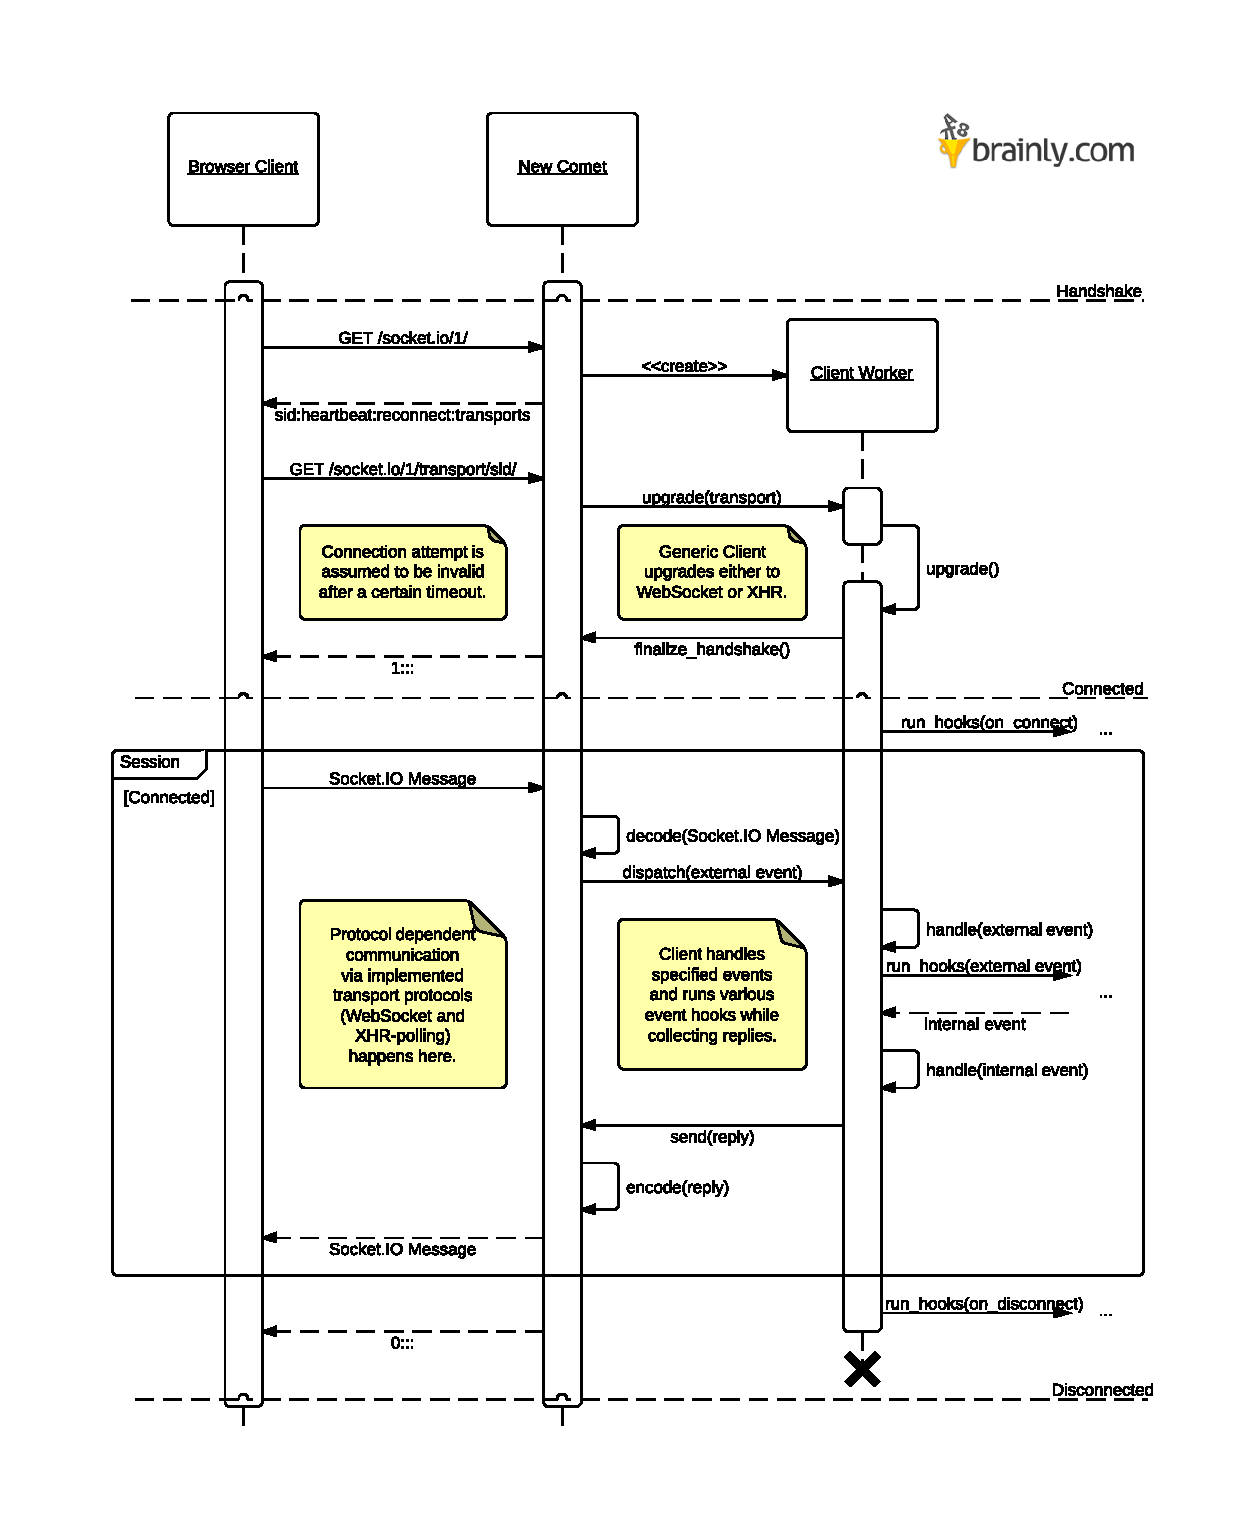
\includegraphics[scale=0.8]{./img/client_server.pdf}
\end{center}

\noindent
Client initializes the connection to the Hive server and receives a Socket.IO handshake response. Next, the client is obliged to attempt to finalize the handshake by sending an initial request to the assigned \textbf{session ID} under a \textbf{transport of his choice}. During the handshake period a \textbf{generic client worker} process is created, which is later upgraded to a \textbf{specific client worker} once a transport has been selected. Connection attempt is assumed invalid after an \textbf{initialization timeout} specified in the configuration file of the Hive server and the client worker is removed.

Once the Socket.IO handshake has been finalized, Client-Server communication may take place. The Client sends Socket.IO messages to the Hive server over the selected transport; the Hive server decodes them into an internal format, routes them to the correct Client worker process (specified by the session ID) and \textbf{handles} them using a \textbf{worker module}. Every such \textbf{external event} (external as in ``outside of the Brainly.com infrastructure'') may trigger several actions of the following types:


\begin{itemize}
\item \textbf{running event hooks} - described in greater detail \hyperref[sec-7-1-4]{here} and \hyperref[sec-9-2]{here}; this may generate \textbf{internal events} (internal as in ``originating from the Brainly.com infrastructure'') which are handled similarly to the external ones, producing replies, state updates or running other event hooks, in turn generating even more internal events,
\item \textbf{updating the client worker state} - described \hyperref[sec-7-1-5]{here},
\item \textbf{sending a reply} - the trivial case, where a reply is sent to the client immediately (this is generally used for Socket.IO control messages, error handling and such).
\end{itemize}

\noindent
If a reply has been generated the Hive server starts polling for a specified amount of time (\textbf{poll timeout}) collecting more replies. Each reply is encoded and fed to the underlying transport handling code, which sends it back to the Client.
If no replies are generated for a specified amount of time (\textbf{heartbeat timeout}) the Hive server will send an empty response to make sure the connection is kept alive.
When a session is terminated (either by the client closing the connection, a session timeout or for any other internal reason, such as receiving a specific internal event) the connection is closed and the Client worker process is terminated.

It is easier to think (and it is the case of the implementation!) that the Client worker acts as a \textbf{finite state machine} with a given set of states and a state transition function. The states are:


\begin{itemize}
\item \textbf{Generic} - a state in which the Client worker is initialized, but not yet finalized; the only valid action for this state is to transition to either of the other states after the client upgrade (upgrade that happens once the Client connects via a specified transport); if the Client fails to finalize the connection in a specified time (\textbf{initialization timeout}), the FSM transitions to the \textbf{Terminated} state,
\item \textbf{Transient} - a ``synchronization'' state where all the Client worker initialization happens; received events are queued in this state and will be handled as soon as the FSM transitions to another state,
\item \textbf{Waiting} - a state in which the Client worker is waiting for external and internal events to handle; events are handled and in case of a \textbf{reply} the FSM transitions to the \textbf{Polling} state,
\item \textbf{Polling} - a state in which the Client worker is collecting more replies to send them as a batch; events are handled and replies are queued; after a specified time (\textbf{poll timeout}) the messages are sent to the Client and the FSM transitions to the \textbf{Waiting} state,
\item \textbf{Terminated} - a state where the Client worker cleans-up after itself and is terminated; no state transitions are valid for this state.
\end{itemize}

\noindent
The state transition scheme outlined above is very general and \emph{not quite true} as it turns out, because different transport protocols require different approaches and special behaviours to be taken care of. For example, \textbf{the sink} (an abstraction representing the underlying transport handling code, where the Client worker \textbf{flushes} the replies) once initialized is always valid for WebSocket, but only until a reply is sent for XHR-polling meaning that XHR-polling clients will occasionally enter the Transient state for short periods of time but the WebSocket ones won't. For this reason the following subsections contain correct and complete state transition diagrams for the concrete Client worker types (currently \textbf{WebSocket} and \textbf{XHR-polling}).


\begin{landscape}
\subsubsection{WebSocket/FlashSocket Client}
\label{sec-7-1-2}

\begin{center}
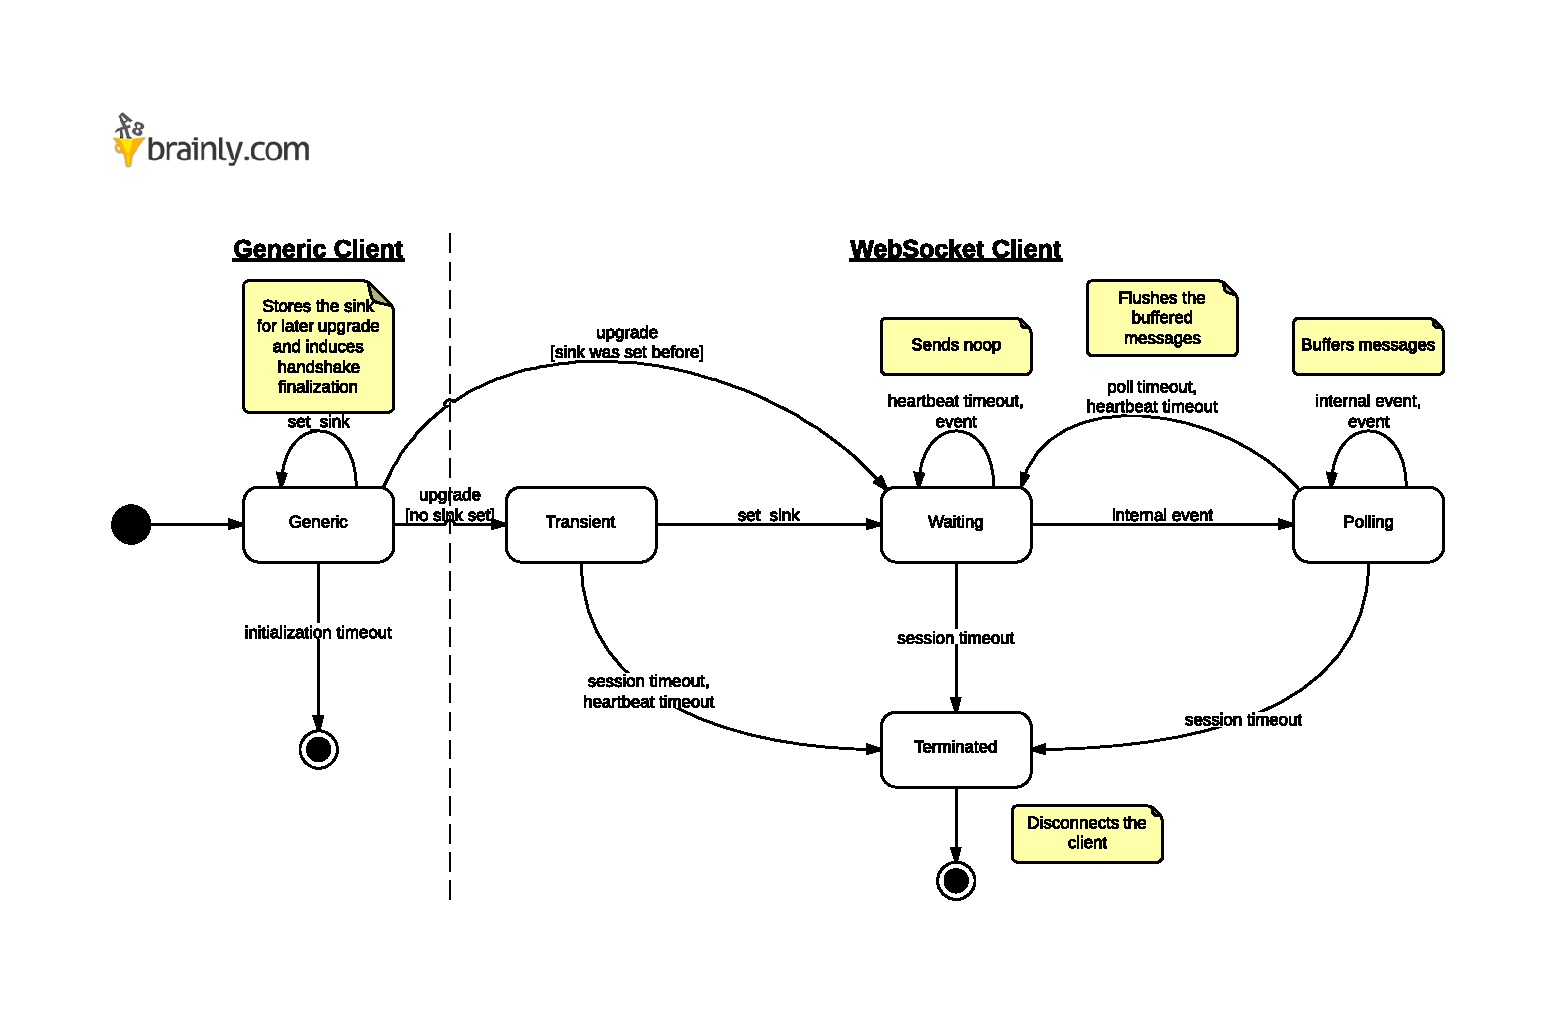
\includegraphics[scale=0.95]{./img/websocket_client.pdf}
\end{center}
\subsubsection{XHR-polling Client}
\label{sec-7-1-3}

\begin{center}
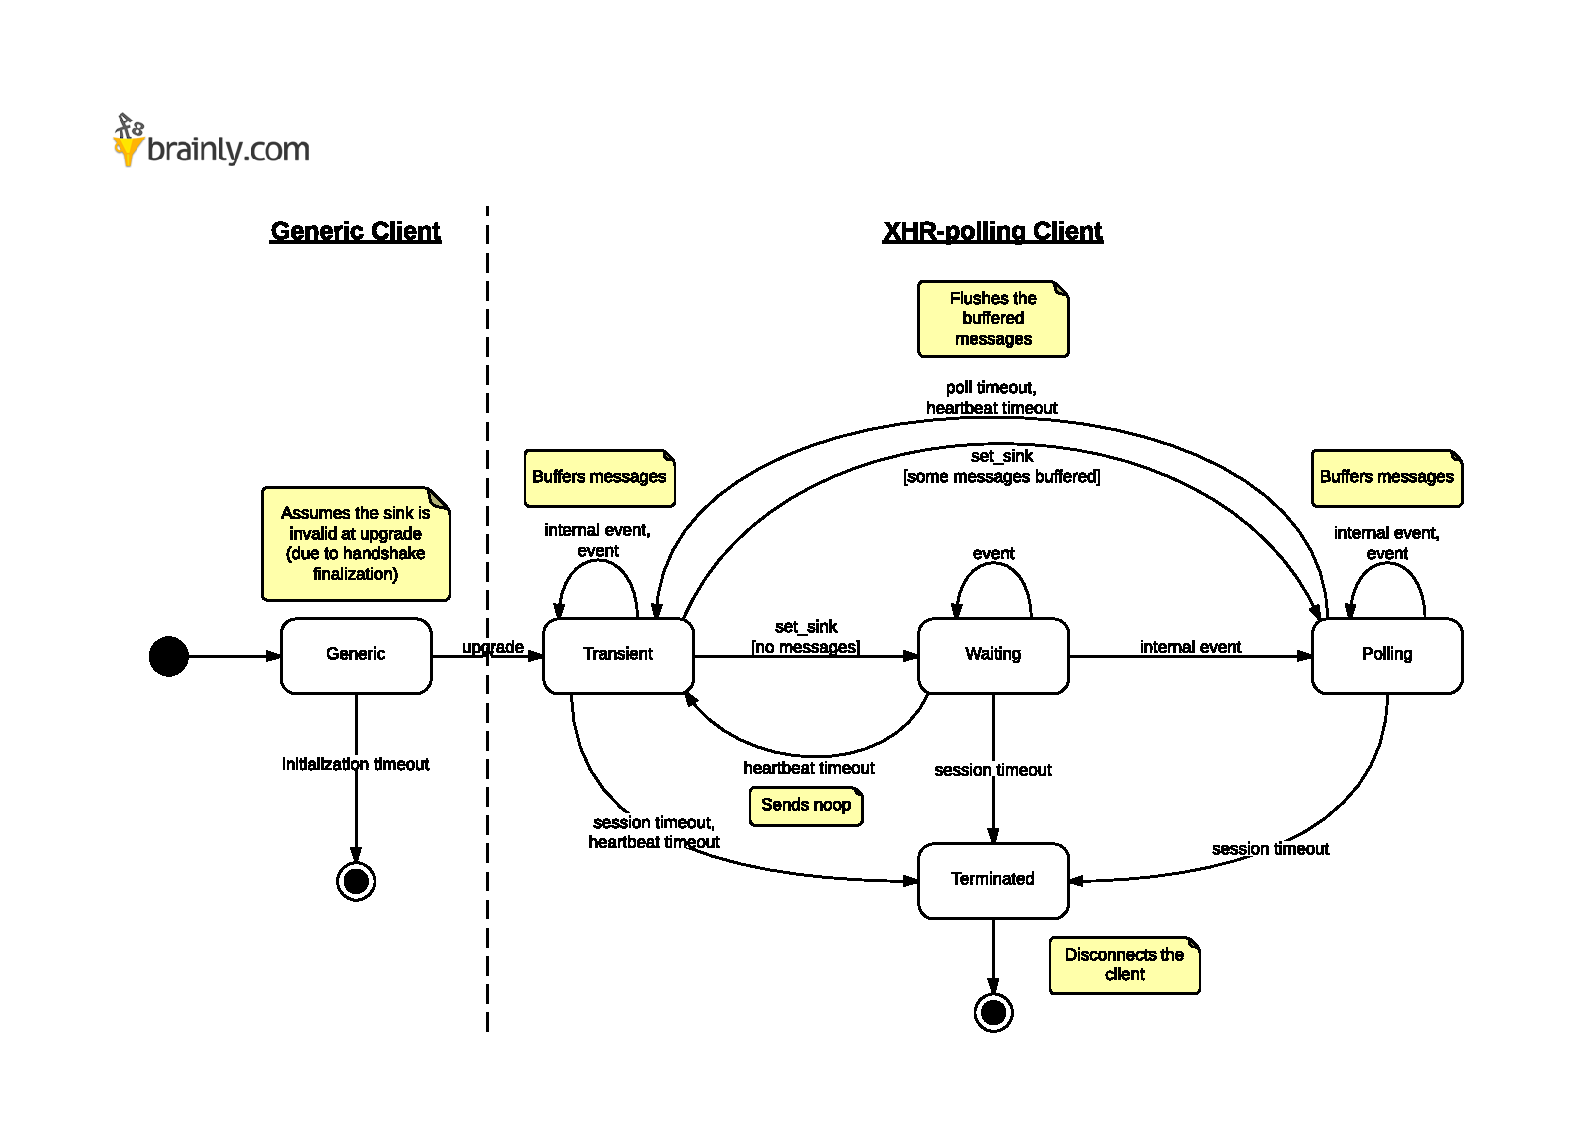
\includegraphics[scale=0.8]{./img/xhr_polling_client.pdf}
\end{center}

\end{landscape}
\subsubsection{Client Hooks}
\label{sec-7-1-4}
\label{ref-client_hooks}

This subsection describes the Hive Hooks facility. Hooks are used to dispatch received \textbf{external} and \textbf{internal events} and perform certain actions based on the event's type and payload.
\begin{itemize}

\item Hook basics\\
\label{sec-7-1-4-1}%
The Hive hooks are defined on a per-event basis, that is, each event type may (or may not) have several hooks associated with it. These hooks will be triggered, and actions they encapsulate will be performed each time an event of that type is received by a Client worker. This holds true for all \textbf{external events} (those originating from the Client) but not for all \textbf{internal events} (those originating from the rest of the system), the later must request further event dispatch (described \hyperref[sec-9-3]{here}). There are several \textbf{special event types} that trigger Hive hooks, that are not received from the Client nor the rest of the system:


\begin{itemize}
\item \texttt{on\_connect} - event generated once the Client worker is upgraded to the final, specialized type; hooks associated with this event \textbf{must not return any replies}, as it is not yet certain that the connection is valid, and sending replies might fail,
\item \texttt{on\_terminate} - event generated on graceful Hive termination; this hook is called shortly before the server termination; any return values are dispatched as normal, but keep in mind that the Client Process \textbf{might be forced to terminate} before any meaningful actions are taken,
\item \texttt{on\_disconnect} - event generated on Client worker termination; any return values of the hooks associated with this event are \textbf{ignored and discarded}.
\end{itemize}

\noindent
Each Hive hook encapsulates a simple action that ts performes upon its invocation. The concrete actions depend on the hook type, and are described in \hyperref[sec-9-2]{a later section}, but a general convention is kept that each action is described in terms of \textbf{metadata}, \textbf{arguments}, \textbf{modification} and \textbf{return values}:


\begin{itemize}
\item Actions receive some Client worker \textbf{metadata} and have it available during execution (more on this \hyperref[sec-7-1-4-2]{later}).
\item Actions take additional \textbf{arguments}, that can be specified in the configuration file.
\item Actions may \textbf{modify} the state of the Client worker during their execution.
\item Actions \textbf{return} one of three result types:
\begin{itemize}
\item \textbf{no reply} - an empty response,
\item \textbf{reply} - returns a reply that will be sent to the Client,
\item \textbf{error} - signalizes an error that will be sent to the Client,
\item \textbf{stop} - stops the hooks execution and terminates the Client worker.
\end{itemize}
\end{itemize}

\noindent
Hooks are run until either of \textbf{stop} or \textbf{error} result is encountered or until there are no more hooks to run. All \textbf{replies} are accumulated and sent to the Client as a batch. Hook order \textbf{does} matter, since each hook might modify the Client workers state, which will be then passed to the next hook in the list.

\noindent
Hook actions may produce \textbf{internal events} that will be dispatched the same way as mentioned \hyperref[sec-9-3]{previously}.

\noindent
Example hook definitions:


\begin{minted}[]{javascript}
"hooks" : {
    "on_connect" : [
        { "hook" : "utils.console_dump", "args" : "Connected!" }
    ],
    "on_disconnect" : [
        { "hook" : "utils.console_dump", "args" : "Disconnected!" }
    ],
    "ping" : [
        { "hook" : "utils.console_dump", "args" : "Pinged!" },
        { "hook" : "utils.echo", "args" : null }
    ],
}
\end{minted}




\noindent
Hooks defined above will cause each Hive Client worker to print ``Connected!'' and ``Disconnected!'' to the console on their initialization and termination respectively. Additionally, a ping event will be logged and echoed back to the Client each time it is received.


\item Client metadata\\
\label{sec-7-1-4-2}%
This subsection describes the metadata used by various Hive Hooks. The metadata consists of the internal state of a Client worker,its Session ID and the event that triggered the hook. It is passed to the hook together with additional arguments defined in the configuration file and it is represented as \textbf{a JSON object} conforming to the following format:


\begin{minted}[]{javascript}
{
    "sid" : "the Session ID of a Client",
    "state" : "the state of the Client worker",
    "trigger" : "the hook-triggering event or null if not present"
    "trigger_id" : "the ACK id of the triggering event"
}
\end{minted}




\noindent
For example:


\begin{minted}[]{javascript}
{
    "sid" : "1238db436e20dbffff182466c8efaa5d757231",
    "trigger" : {
        "name" : "ping",
        "args" : ["pong"]
    },
    "trigger_id" : "1+",
    "state" : {
        "initial_value" : null
    }
}
\end{minted}





\item Hooks summary\\
\label{sec-7-1-4-3}%
The Client worker/hook interaction is summarized on the following diagram:

\begin{center}
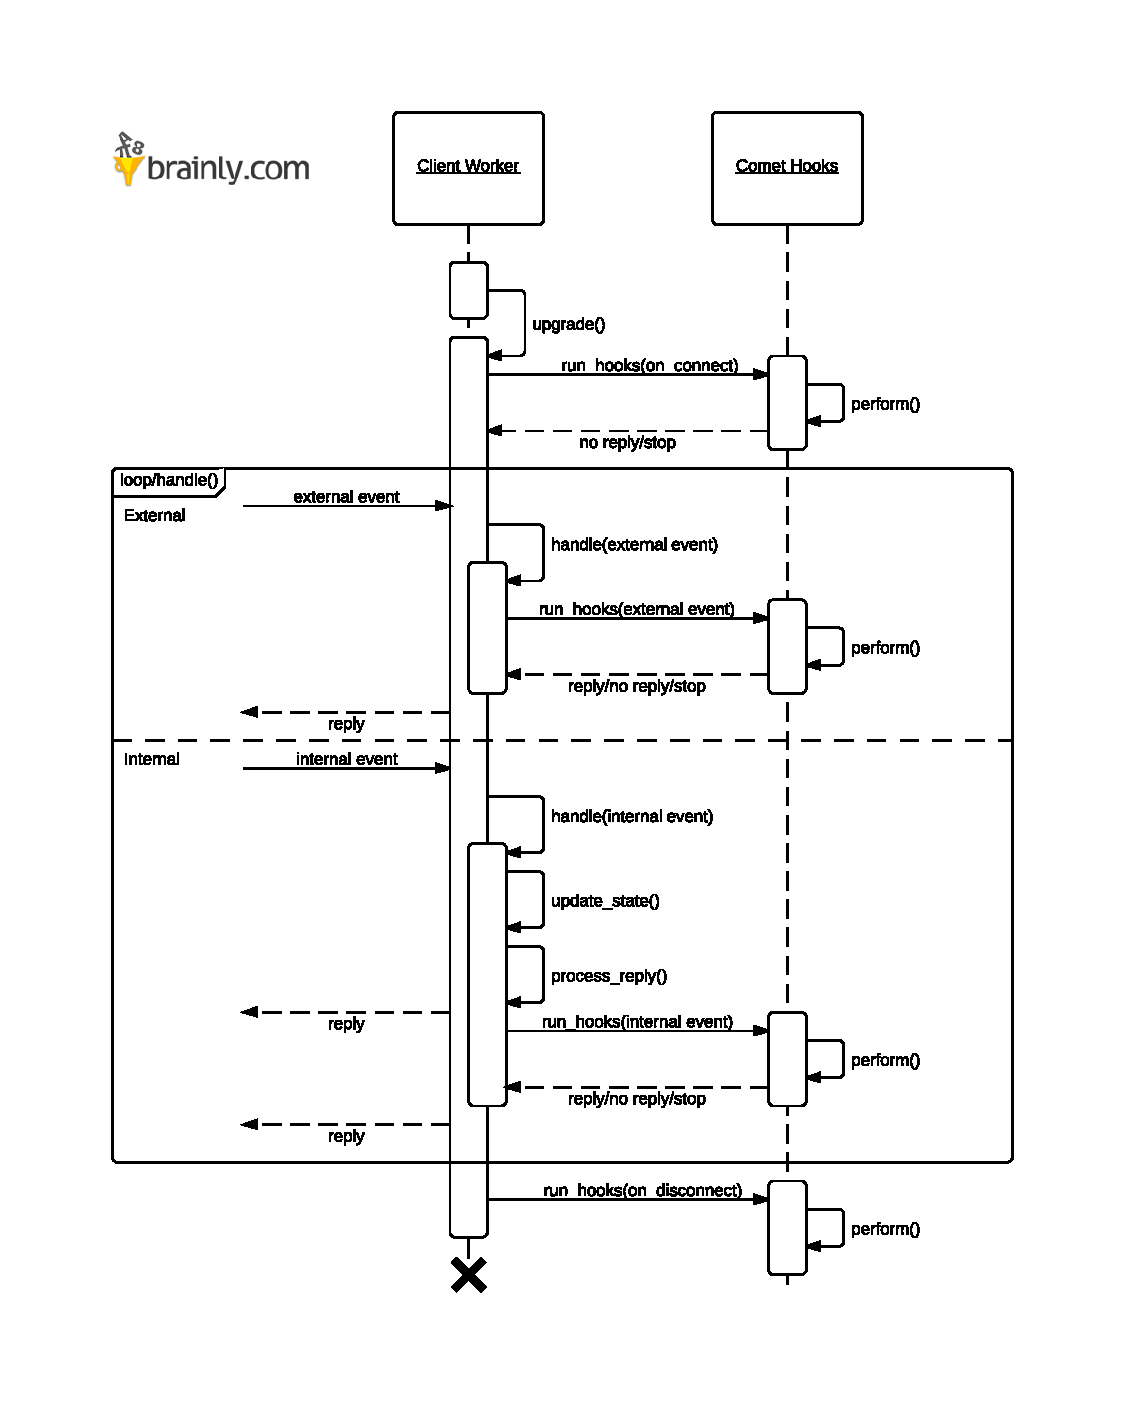
\includegraphics[scale=0.9]{./img/client_hooks.pdf}
\end{center}

\end{itemize} % ends low level
\subsubsection{Client state management}
\label{sec-7-1-5}
\label{ref-state_management}

This subsection describes the Client State Manager - a facility used to manage the Client worker state as a key-value store. Most of the technical details have been omitted for various reasons.

\noindent
The configuration file has to specify \textbf{a state manager descriptor}, which defines several fields:


\begin{minted}[]{javascript}
{
    "state_manager" : "The name of the State Manager to use, e.g. sm.redis.",
    "initial_value" : "Initial state of the Client.",
    "args" : "Additional arguments required by the State Manager."
}
\end{minted}




The \texttt{initial\_value} may be \textbf{any JSON value}, however since the State Manager provides a key-value store interface, JSON objects are treated as lists of key-value pairs with each value stored at each key, and values other than JSON objects are stored using \texttt{initial\_value} key. For example:


\begin{minted}[]{javascript}
"initial_value" : {"foo" : "bar", "bar" : "baz"} // Stored as:  foo:bar, bar:baz
"initial_value" : [1, 2, 3]                      // Stored as: initial_value:[1, 2, 3]
"initial_value" : "foo"                          // Stored as: initial_value:foo
\end{minted}




\noindent
A list all available State Managers and their configuration parameters can be found \hyperref[sec-9-5]{here}.

\pagebreak
\subsection{Service Connectors}
\label{sec-7-2}

This section describes other details of the Hive Connectors facility. The Hive Connectors facility that provides access to various services, such as Redis databases or HTTP servers, uses several schemes of worker pool management. A pool consists of a supervisor and a number of \textbf{worker processes}, which are \textbf{rented} by various other Hive modules (for example Hive Protocol hooks). Technical details of pool management and worker renting were omitted from this user guide.

Each pool can be \textbf{named} and has a configurable size that may increase temporarily during run-time, therefore each pool can be described in terms of its \textbf{name}, a \textbf{connector plugin}, \textbf{size} and \textbf{overflow} (the maximum number of additional worker processes to spawn under heavy server load) and \textbf{arguments} it uses for set-up, which, incidentally, are the configuration parameters required by each Hive Connectors pool.

\noindent
A list all available Connector pools can be found \hyperref[sec-9-4]{here}.
\subsubsection{Connectors summary}
\label{sec-7-2-1}

The Client worker/Connector pool interaction is summarized on the following diagram:

\begin{center}
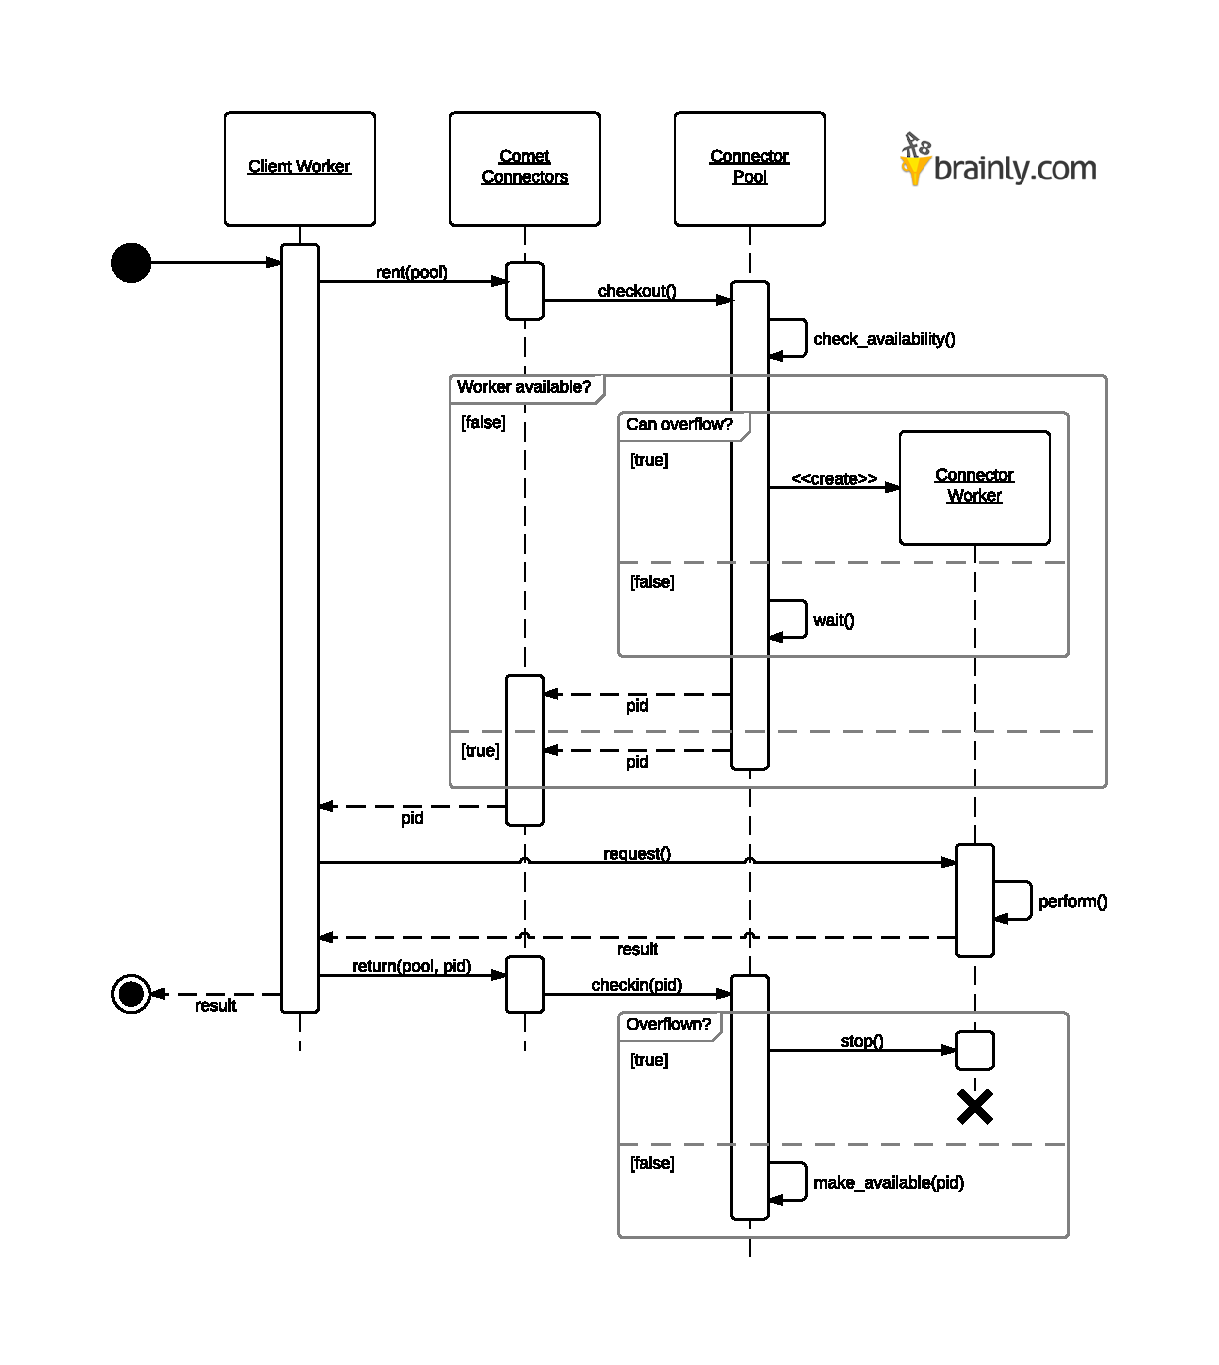
\includegraphics[scale=0.9]{./img/connectors.pdf}
\end{center}

\pagebreak
\subsection{Pub-Sub Channels}
\label{sec-7-3}
\label{ref-pubsub}

This subsection and its subsections describe the Hive Pub-Sub facility.
\subsubsection{Channel templates}
\label{sec-7-3-1}

A set of Pub-Sub channel templates can be defined in the Hive configuration file. Each template consists of a \textbf{channel prefix} - the first part of the channel ID, and a \textbf{channel descriptor} - as described \hyperref[ref-pubsub_config]{here}. At runtime, channels are created using one of the templates determined by their channel ID. Any attempt at creating a channel that doesn't follow any channel template defined in the configuration file will fail and an error response will be produced.
\subsubsection{Channel types}
\label{sec-7-3-2}

Each template defines a channel type. Hive Pub-Sub currently supports two types of channels:


\begin{itemize}
\item \textbf{private} channels - accesible only via the Hive API Server or via Client Pub-Sub Hook with a sufficient privilege level.
\item \textbf{public} channels - accessible by all Clients.
\end{itemize}
\subsubsection{Channel management}
\label{sec-7-3-3}

Each Pub-Sub channel is created with the first Client attempting a subscription. As long as there are Clients subscribed to a channel it'll stay active and publish messages to its subscribents. When the last Client unsubscribes from the channel, depending on the timeout that was configured for the correspording channel template, the channel might expire and cease to exist, or continue waiting for more subscribents.

\noindent
Channel (un)subscriptions can be managed in either of the following ways:


\begin{itemize}
\item via the Hive API Server - as described \hyperref[sec-6-1-7]{here},
\item via the Hive Pub-Sub Hook - as described \hyperref[sec-9-2-4]{here}.
\end{itemize}

\noindent
Events can be published to the Hive Pub-Sub channel only via the Hive API Server (as described \hyperref[sec-6-1-7]{here}).
\subsubsection{Pub-Sub summary}
\label{sec-7-3-4}

The following diagrams summarize the Hive Pub-Sub channel operation.

\pagebreak
\begin{landscape}
\begin{itemize}

\item Hive API Server subscription:
\label{sec-7-3-4-1}%
\begin{center}
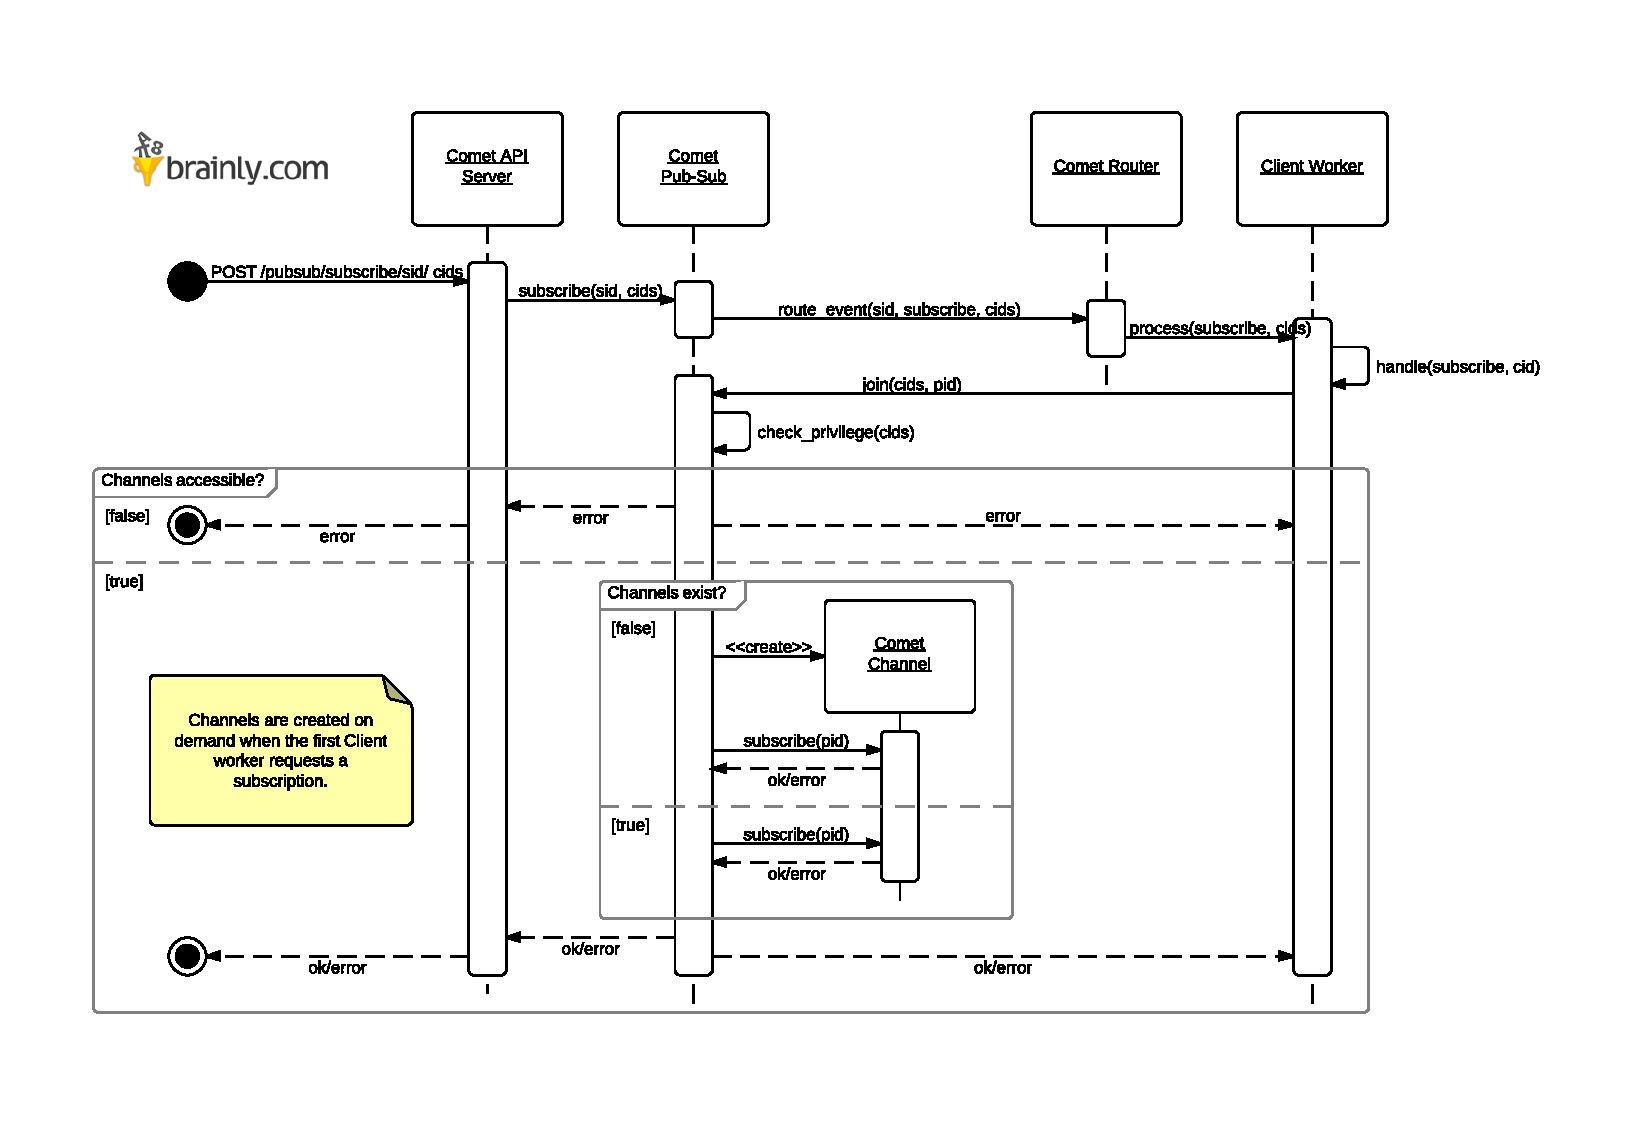
\includegraphics[scale=0.85]{./img/pubsub_api_subscription.pdf}
\end{center}

\pagebreak

\item Hive API Server unsubscription:
\label{sec-7-3-4-2}%
\begin{center}
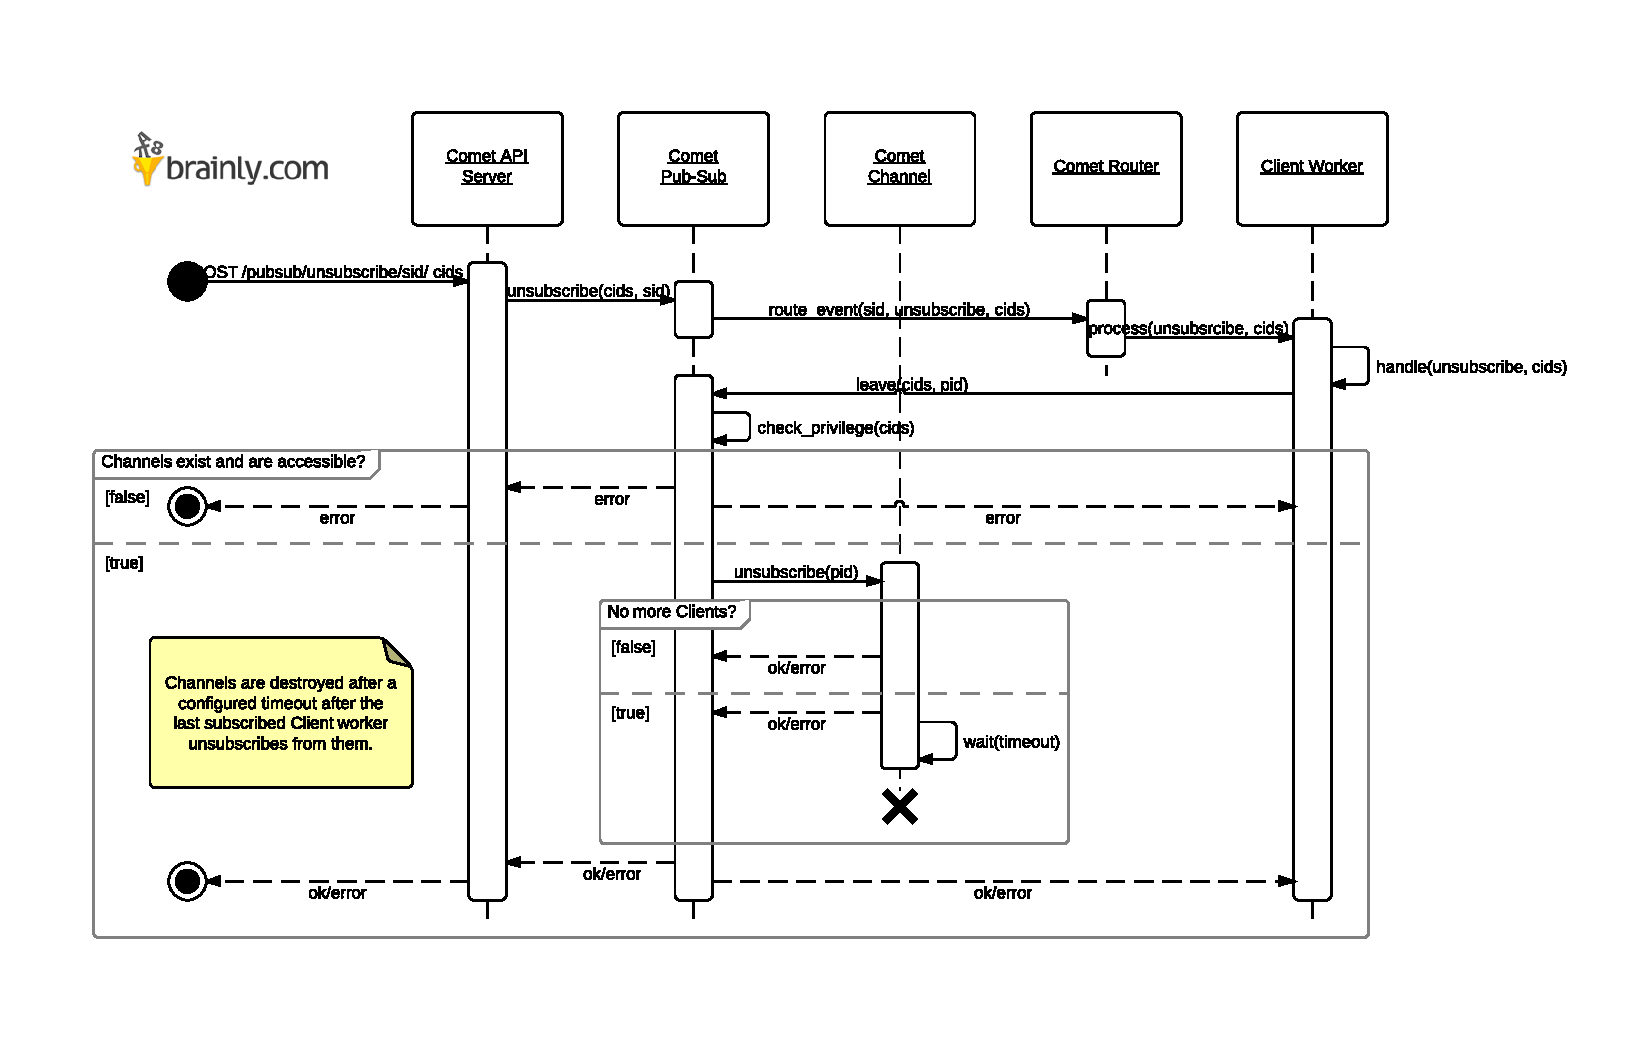
\includegraphics[scale=0.9]{./img/pubsub_api_unsubscription.pdf}
\end{center}

\pagebreak


\item Hive API Server publishing:
\label{sec-7-3-4-3}%
\begin{center}
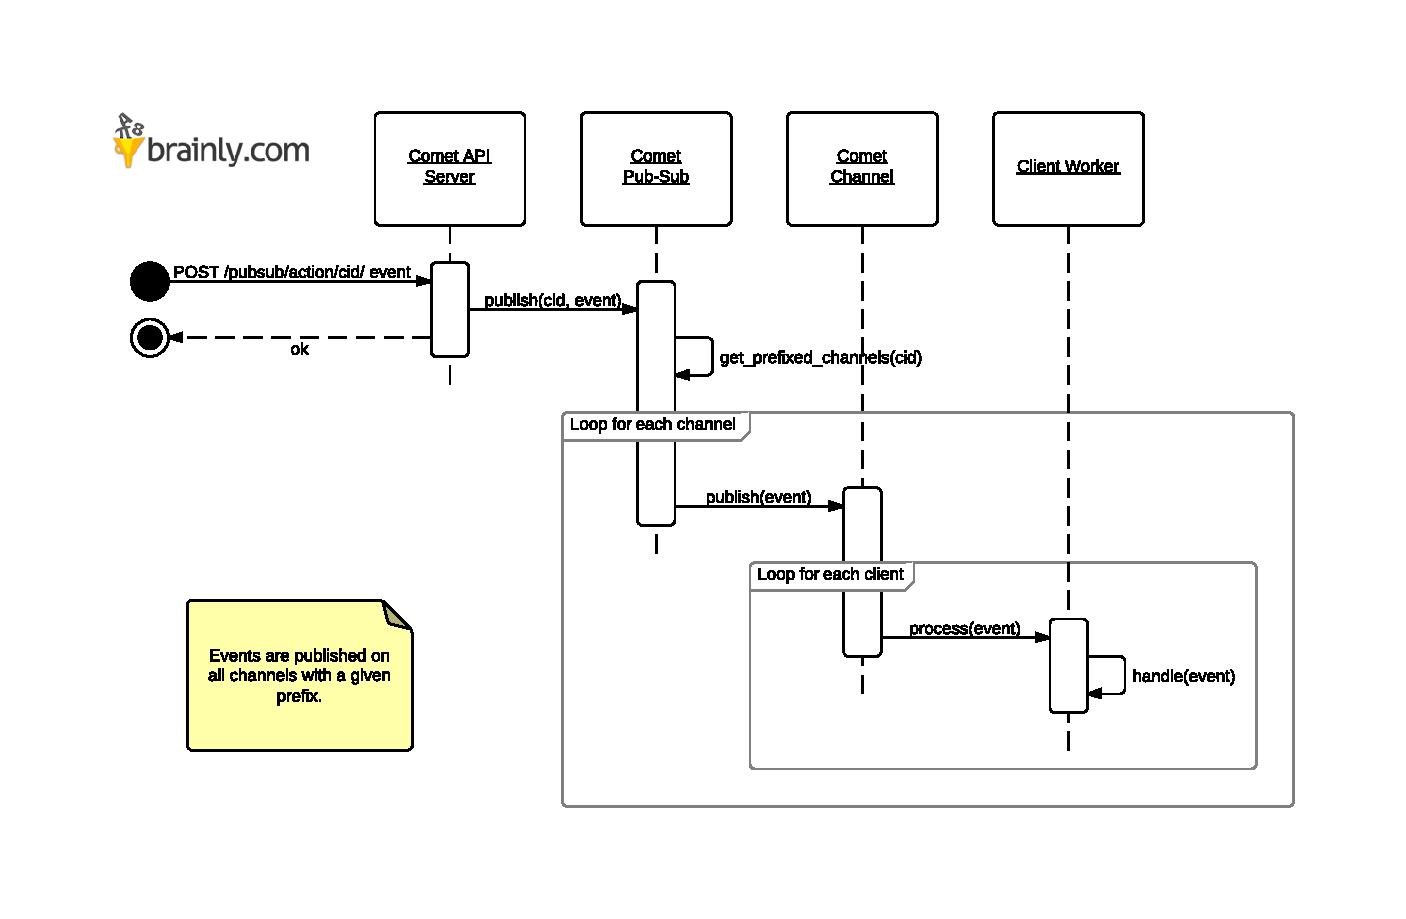
\includegraphics[scale=1.0]{./img/pubsub_api_publishing.pdf}
\end{center}

\pagebreak

\item Hive API Server raw-publishing:
\label{sec-7-3-4-4}%
\begin{center}
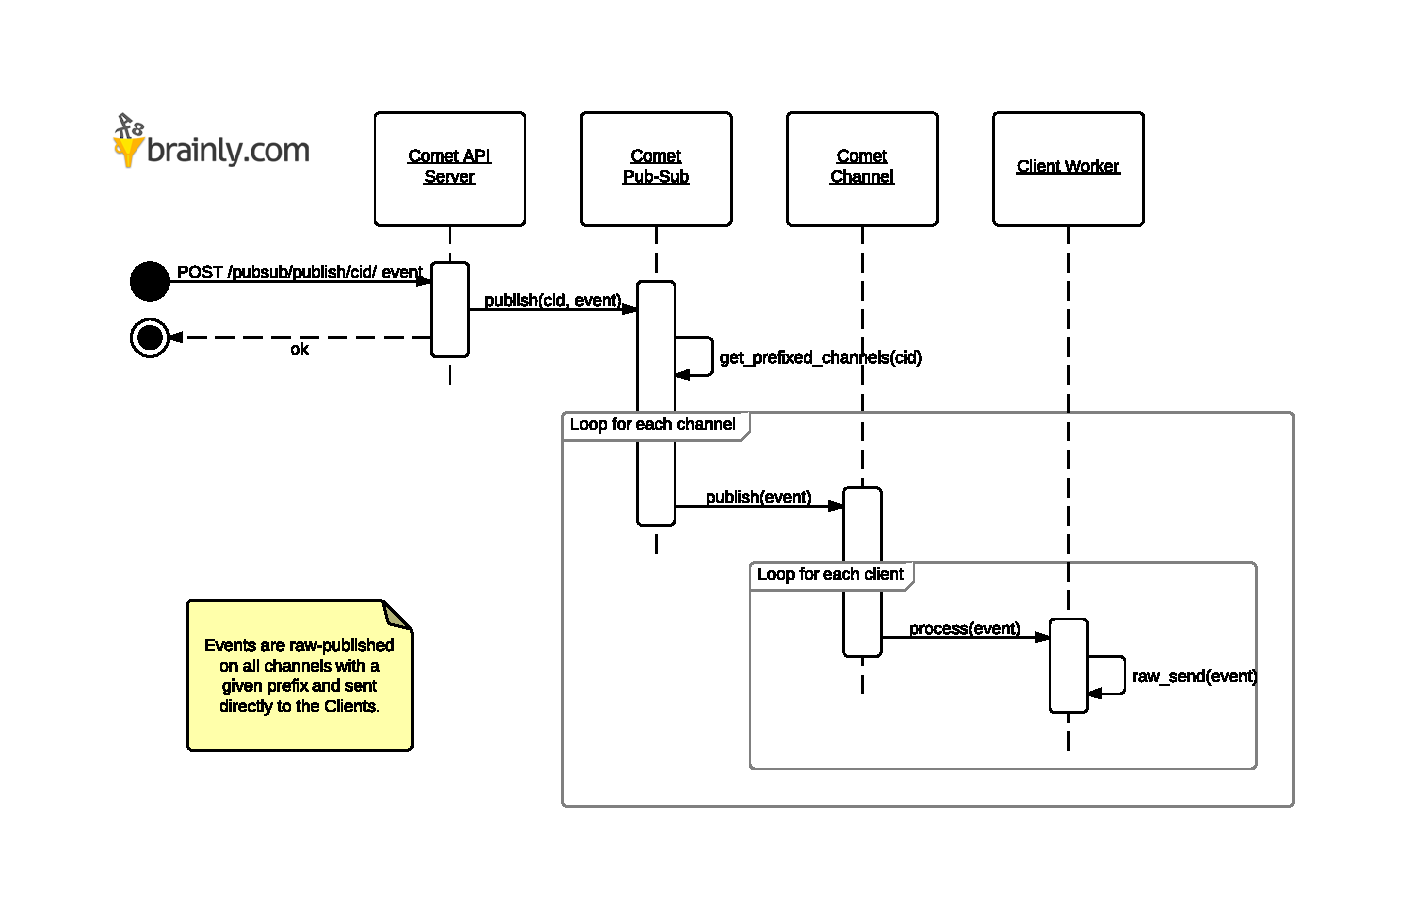
\includegraphics[scale=1.0]{./img/pubsub_api_raw_publishing.pdf}
\end{center}

\pagebreak

\item Hive Client Worker subscription:
\label{sec-7-3-4-5}%
\begin{center}
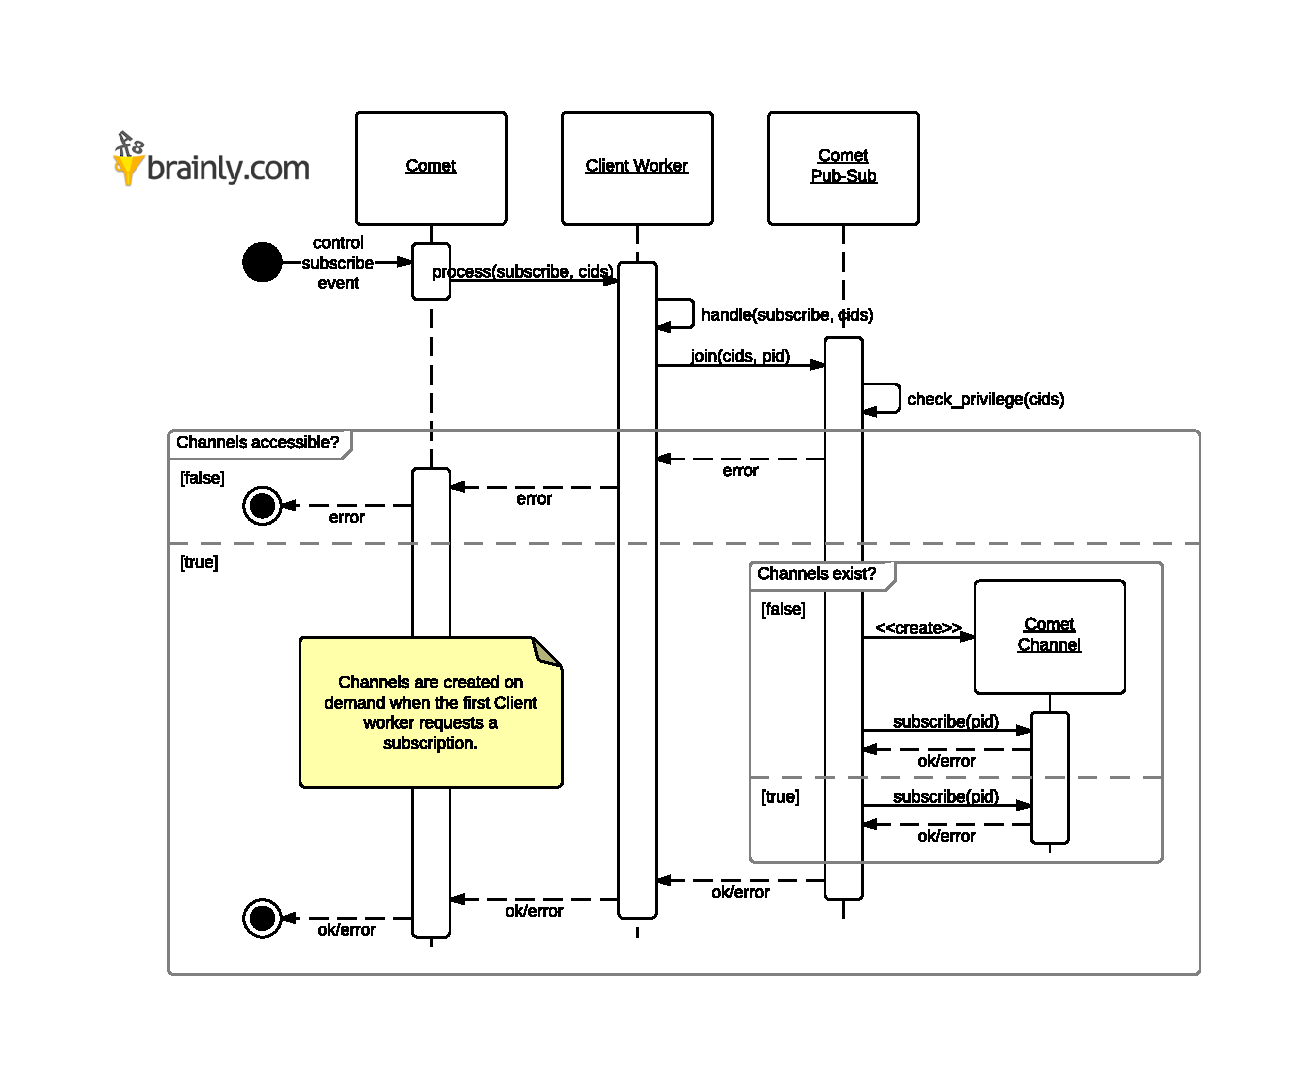
\includegraphics[scale=0.85]{./img/pubsub_client_subscription.pdf}
\end{center}

\pagebreak

\item Hive Client worker unsubscription:
\label{sec-7-3-4-6}%
\begin{center}
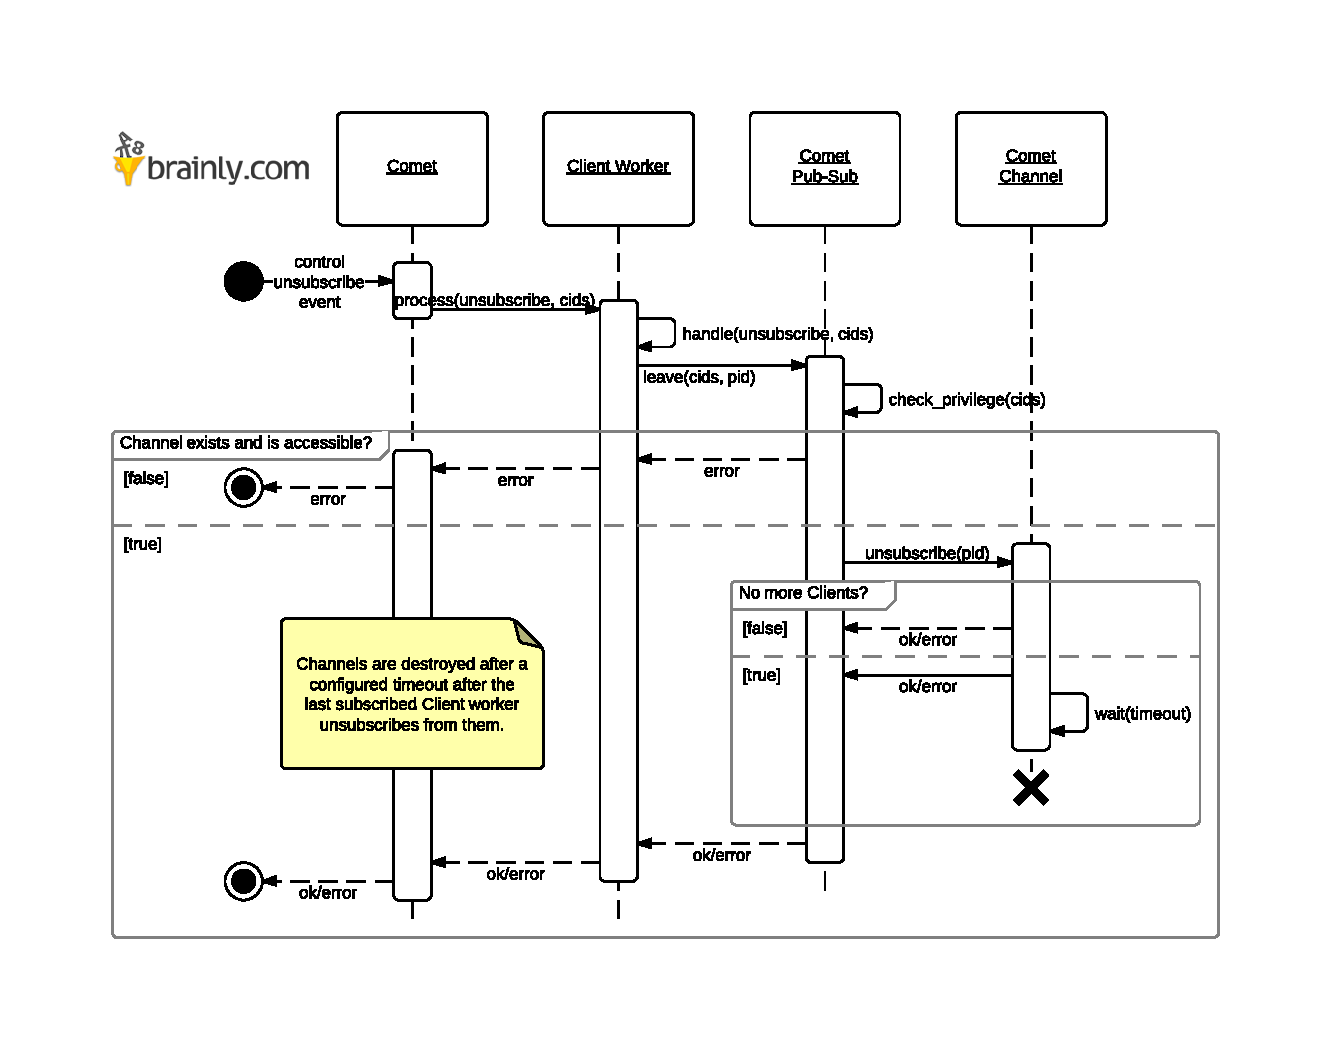
\includegraphics[scale=0.90]{./img/pubsub_client_unsubscription.pdf}
\end{center}

\end{landscape}
\pagebreak

\end{itemize} % ends low level
\subsection{Non-Erlang modules}
\label{sec-7-4}

The Hive server may be combined with a number of modules written in non-Erlang programming languages for convenience and easy integration with existing backends. All that is needed is a little Hive Protocol conformance on the backend side.
\subsubsection{Hive Protocol basics}
\label{sec-7-4-1}

The \textbf{Hive Protocol} is a set of communication rules and data formats that are recognized by the Hive server. It involves three components:


\begin{itemize}
\item \textbf{Internal Events} \& \textbf{Client Metadata JSON} - described in detail \hyperref[sec-9-3]{here} and \hyperref[sec-7-1-4-2]{here}.
\item \textbf{Hive Protocol hook} - described in detail \hyperref[sec-9-2-8]{here}.
\item \textbf{Hive API} - described in detail \hyperref[sec-6]{previously}.
\end{itemize}

\noindent
Hive Protocol communication is either \textbf{simplex} or \textbf{duplex}:

\begin{itemize}
\item Simplex communication on the Hive-Backend path results in Client Metadata being sent to the Backend.
\item Simplex communication on the Backend-Hive path results in Internal Events being dispatched on vaia Hive API calls.
\item Duplex communication on the Hive-Backend path results in Client Metadata being sent to the Backend and Internal Events being received from the Backend as a response. This is the only duplex communication in the Hive Protocol.
\end{itemize}

\noindent
An example of a Hive Protocol based communication is presented below:


\begin{minted}[]{javascript}
// Browser Client sends an event:
{
    "name" : "ping",
    "args" : []
}

// Hive Worker dispatches on the event
// using ping hook configured as follows:
"ping" : [
    {
        "hook" : "hp.post",
        "args" : {
            "endpoint" : "ping.php",
            "connector" : "php_backend"
        }
    }
]

// A Client Metadata JSON is passed to the backend via
// php_backend connector in a POST request:
{
    "sid" : "client_id",
    "trigger" : {
        "name" : "ping",
        "args" : []
    },
    "trigger_id" : "",
    "state" : {
        "initial_value" : null
    }
}

// The backend processes the request and generates a reply:
{
    "action" : "reply",
    "args" : {
        "name" : "pong",
        "args" : ["one"]
    }
}

// The backend proceeds to send more events via
// a request to Hive API /client/action/client_id endpoint:
{
    "action" : "reply",
    "args" : {
        "name" : "pong",
        "args" : ["two"]
    }
}

// The Hive API passes the event to the Client Worker.

// The Client worker dispatches on the replies
// using reply dispatcher configured as follows:
"reply" : [
    {
        "action" : "action.send_event",
        "args" : null
    }
]

// Both replies are sent to the Browser client:
{
    "name" : "pong",
    "args" : ["one"]
},
{
    "name" : "pong",
    "args" : ["two"]
}
\end{minted}
\subsubsection{Non-Erlang modules summary}
\label{sec-7-4-2}

The Hive-Backend interaction is somewhat simplistic. It uses all of the major built-it Hive facilities such as the \hyperref[sec-7-1-4]{Hive Hooks}, \hyperref[sec-9-3]{Hive Internal Event dispatchers} and \hyperref[sec-6]{Hive API servers} and can be divided into two itertwinded flows that run simultaneously


\begin{itemize}
\item \textbf{the Event loop} - this is a reactive event loop where \textbf{external events} originating from the Clients are dispatched resulting in \textbf{Hive Protocol Hooks} invocations and Hive-Backend communication.
\item \textbf{the API loop} - this is a proactive loop where \textbf{API calls} originating from the Backend are handled what may result in a number of \textbf{Internal Event dispatchers} invocations and Hive-Browser communication.
\end{itemize}

\noindent
The Hive-Backend interaction has been summarized on the following diagram:

\begin{center}
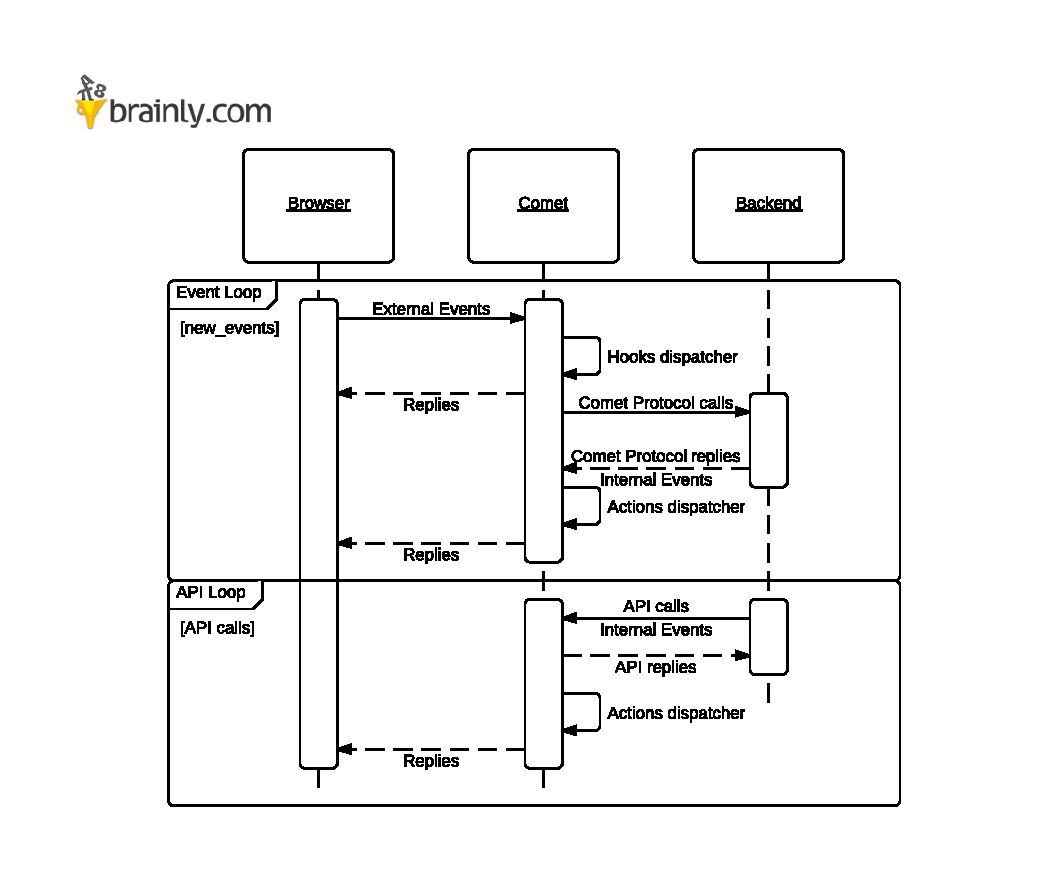
\includegraphics[scale=1.0]{./img/hive_usage.pdf}
\end{center}

\pagebreak
\section{Clusterization}
\label{sec-8}
\label{ref-cluster}

Hive can be configured to run in a cluster, where various messages are propagated between several nodes to achieve some transparency of operation - for example, \hyperref[sec-7-3]{Pub-Sub channels}, even though distributed between several nodes, will act as a single facility, transparently forwarding messages to any connected clients.
The following subsections sketch Hive clusterization and give some hints on Cluster naming convention and internal communication.
\subsection{Clusterization basics}
\label{sec-8-1}

In order to clusterize Hive you have to \hyperref[ref-cluster-config]{configure} relevant parameters and run several instances of the server. Everything else will be handled for you automatically. Instances need to know about at least one of currently live cluster nodes in order to successfully join a cluster.

Every node in a Hive cluster is of the same rank, there is no distinction into master or slave nodes. This means that the cluster can be easily resized at run-time simply by starting new Hive instances which are configured to connect to any of the already running nodes.

Each newly connected node will automatically start receiving all necessary messages comming from the rest of the Cluster and it'll act accordingly.
\subsection{Cluster naming convention}
\label{sec-8-2}
\label{ref-cluster-naming-convention}


Each Hive node has to be given a name in order to successfully form or join a cluster. The node name syntax is as follows:


\begin{minted}[]{javascript}
IDPart [ '@' ( HostPart '.' DomainPart | IPAddress ) ]
\end{minted}




The address part names the machine Hive is running on, usually this will be an \texttt{IPAddress}, but a \textbf{fully qualified domain name} can be used.
The address part is optional in the configuration file - when left out, Hive will attempt to infere it from your hosts configuration. If inference is successful, the \texttt{HostPart} will contain the host name of your machine, and the \texttt{DomainPart} will contain the domain associated with your machines IP address.

The \texttt{IDPart} is a short identificator of the particular Hive instance, it doesn't have to be unique as long as the entire name is unique.

Similarily, the Hive Cluster has to be given a name in order for each Hive instance to identify other cluster members. The cluster name is largely arbitrary as long as it's a non-empty string.
\subsection{Cluster-wide communication}
\label{sec-8-3}

Currently, Hive nodes propagate several types of messages throughout the Hive Cluster:


\begin{itemize}
\item any Internal Events routed using the Hive Router,
\item any Internal Events routed using the Hive Pub-Sub facility - but only on the Pub-Sub Manager level, each Pub-Sub Channel propagates messages to the Clients locally.
\end{itemize}

Additionally, Hive nodes will broadcast some messages in order to maintain the Cluster structure. These include:


\begin{itemize}
\item heartbeats,
\item status updates,
\item connection/disconnection notifications.
\end{itemize}

\pagebreak
\section{Hive Plugins}
\label{sec-9}
\label{ref-plugins}

Hive Plugins framework is an elaborate way to define extentions for the Hive server. Detailed description of the Hive Plugins framework is outside of the scope of this document. This section describes the Hive Plugins framework and gives a brief description of the available built-in plugins.
\subsection{Plugins basics}
\label{sec-9-1}

Hive Plugins reside in the \textbf{plugins} directory and are written in the Erlang programming language. Plugins are \emph{loosely} structured and do not have to reside in a single module, however plugins must follow several conventions:

\noindent
The \textbf{type convention} - Hive server supports currently for types of plugins that differ in their API:


\begin{itemize}
\item \textbf{State Managers} - manage the state of the Hive Workers,
\item \textbf{Hooks} - allow the Hive Workers to perform some actions,
\item \textbf{Internal Events} - allow the backend to control the Hive Workers,
\item \textbf{Service Connectors} - provide the means to connect to various services.
\end{itemize}

\noindent
The \textbf{API convention} - Hive server defines a common Hive Plugin API in addition to the specific plugin-type API that allows for an automated plugins loading during Hive startup:


\begin{itemize}
\item \textbf{load} - loads plugins from a plugin-module and performs all necessary initial checks; there may be several plugins defined in a single plugin module,
\item \textbf{validate} - validates plugin configuration and performs all additional checks,
\item \textbf{unload} - unloads a plugin and performs all necessary cleanup.
\end{itemize}

\noindent
And least importantly, the \textbf{naming convention} - plugins once loaded reside in a common namespace. Some care must be taken to avoid name clashes. Generally, the following naming convention is used:


\begin{itemize}
\item \textbf{sm.plugin} - names a State Manager,
\item \textbf{purpose.plugin} - names a Hook that serves some \textbf{purpose},
\item \textbf{action.plugin} - names an Internal Event dispatcher,
\item \textbf{connector.plugin} - names a Service Connector.
\end{itemize}

\noindent
Every plugin expects to receive a configuration descriptor on initialization. The descriptor should be of the following format (``type'' is either \texttt{connector}, \texttt{state\_manager}, \texttt{hook} or \texttt{event} depending on the plugin type):


\begin{minted}[]{javascript}
{
    "type" : "plugin",
    "args" : "Additional arguments",
    "additional" : "fields",
    ...
}
\end{minted}




\noindent
The built-in plugins are described shortly in the following subsections.
\subsection{Client Hooks}
\label{sec-9-2}
\label{ref-hooks}
\subsubsection{\texttt{utils.echo}}
\label{sec-9-2-1}


Echoes any received Socket.IO messages back to the Client.


\begin{itemize}
\item metadata used - none,
\item arguments taken - either none or \textbf{an external event} to reply with,
\item modifications to the state - none,
\item results in - \textbf{always replies} with a Socket.IO message.
\end{itemize}

\noindent
Example declarations:

\begin{minted}[]{javascript}
{ "hook" : "utils.echo", "args" : null }
{ "hook" : "utils.echo", "args" : { "name" : "event", "args" : "arguments" } }
\end{minted}
\subsubsection{\texttt{utils.console\_dump}}
\label{sec-9-2-2}

Dumps the state of a Client worker to the console together with a distinct message passed as an argument. Meant for debugging purposes.


\begin{itemize}
\item metadata used - the Client workers internal state (Session ID, stored values, event that triggered the hook),
\item arguments taken - a short message to be printed in the console; has to be \textbf{a string},
\item modifications to the state - none (but accesses the stored values),
\item results in - \textbf{never replies nor stops}.
\end{itemize}

\noindent
Example declaration:

\begin{minted}[]{javascript}
{ "hook" : "utils.console_dump", "args" : "Hello Hive!" }
\end{minted}
\subsubsection{\texttt{utils.dispatch}}
\label{sec-9-2-3}

Dispatches on the triggering external event as if it were an interternal one.


\begin{itemize}
\item metadata used - the Client workers internal state (Session ID, stored values, event that triggered the hook),
\item arguments taken - none,
\item modifications to the state - may modify anything as it treats the triggering event as an internal event,
\item results in - might return either \textbf{reply}, \textbf{no reply} or even stop the Client worker.
\end{itemize}

\noindent
Example declaration:

\begin{minted}[]{javascript}
{ "hook" : "utils.dispatch", "args" : null }
\end{minted}
\subsubsection{\texttt{pubsub.subscribe}}
\label{sec-9-2-4}
\label{ref-hook_pubsub}


Subscribes a Client to the Hive Pub-Sub channels specified in arguments of the triggering event.


\begin{itemize}
\item metadata used - the Client workers internal state (Session ID, stored values, event that triggered the hook),
\item arguments taken - \textbf{a string} representing the privilege level of this hook,
\item modifications to the state - none,
\item results in - does \textbf{not reply}, might stop the Client worker in case of a failure.
\end{itemize}

\noindent
Example declaration:

\begin{minted}[]{javascript}
{ "hook" : "pubsub.subscribe", "args" : "public" }
\end{minted}




\noindent
Example triggering event (causes subscription to channels \texttt{foo.bar.baz}, \texttt{faz.baz} and \texttt{fez}):


\begin{minted}[]{javascript}
{
    "name" : "subscribe",
    "args" : [
        {
            "foo" : {
                "bar" : ["baz"]
            },
            "faz" : "baz"
        },
        "fez"
    ]
}
\end{minted}
\subsubsection{\texttt{pubsub.resubscribe}}
\label{sec-9-2-5}

First attempts to leave all subscribed channels matching prefixes given in the triggering event and then resubscribes the Client to all specified, concrete channel IDs.


\begin{itemize}
\item metadata used - the Client workers internal state (Session ID, stored values, event that triggered the hook),
\item arguments taken - \textbf{a string} representing the privilege level of this hook,
\item modifications to the state - none,
\item results in - does \textbf{not reply}, might stop the Client worker in case of a failure.
\end{itemize}

\noindent
Example declaration:

\begin{minted}[]{javascript}
{ "hook" : "pubsub.resubscribe", "args" : "public" }
\end{minted}




\noindent
Example triggering event (causes subscription to channels \texttt{foo.bar.baz}, \texttt{faz.baz} and \texttt{fez}):


\begin{minted}[]{javascript}
{
    "name" : "resubscribe",
    "args" : [
        {
            "prefxi_1" : {
                "bar" : ["baz"]
            },
            "prefix_2" : "baz"
        }
    ]
}
\end{minted}
\subsubsection{\texttt{pubsub.unsubscribe}}
\label{sec-9-2-6}


Unsubscribes a Client from the Hive Pub-Sub channels specified in arguments of the triggering event.


\begin{itemize}
\item metadata used - the Client workers internal state (Session ID, stored values, event that triggered the hook),
\item arguments taken - \textbf{a string} representing the privilege level of this hook,
\item modifications to the state - none,
\item results in - does \textbf{not reply}, might stop the Client worker in case of a failure.
\end{itemize}

\noindent
Example declaration:

\begin{minted}[]{javascript}
{ "hook" : "pubsub.unsubscribe", "args" : "public" }
\end{minted}




\noindent
Example triggering event (causes unsubscription from channels \texttt{foo.bar.baz}, \texttt{faz.baz} and \texttt{fez}):


\begin{minted}[]{javascript}
{
    "name" : "subscribe",
    "args" : [
        {
            "foo" : {
                "bar" : ["baz"]
            },
            "faz" : "baz"
        },
        "fez"
    ]
}
\end{minted}
\subsubsection{\texttt{pubsub.publish}}
\label{sec-9-2-7}


Publishes internal events passed as the arguments of the triggering event on a Hive Pub-Sub channels specified in arguments.


\begin{itemize}
\item metadata used - the Client workers internal state (Session ID, stored values, event that triggered the hook),
\item arguments taken - \textbf{a JSON object} containing the Hive Pub-Sub channel IDs and the privilege level of this hook,
\item modifications to the state - none,
\item results in - does \textbf{not reply}, might stop the Client worker in case of a failure.
\end{itemize}

\noindent
Example declaration:

\begin{minted}[]{javascript}
{
    "hook" : "pubsub.publish",
    "args" : {
        "cids" : ["foo", "bar"],
        "privilege" : "public"
    }
}
\end{minted}




\noindent
Example triggering event (causes the Client to publish events on Hive Pub-Sub channels \texttt{foo} and \texttt{bar}):


\begin{minted}[]{javascript}
{
    "name" : "publish",
    "args" : [
        { "action" : "event1", "args" : "arguments" },
        ...
    ]
}
\end{minted}
\subsubsection{\texttt{hp.get}}
\label{sec-9-2-8}
\label{ref-hive_protocol_hook}

Performs a synchronous request, similar in semantics to an HTTP GET, to a given endpoint using a given Hive Protocol compatible Hive Connector pool (listed \hyperref[ref-cp_connector]{here}).


\begin{itemize}
\item metadata used - none,
\item arguments taken - \textbf{a JSON object} that contains: \textbf{endpoint} - a string representing the endpoint, \textbf{connector} - name of the Hive Protocol compatible Hive Connectors pool to use.
\item modifications to the state - none,
\item results in - dispatches the reply immediately and may \textbf{not reply}, \textbf{reply}, \textbf{error} or even \textbf{stop} the Client worker.
\end{itemize}

\noindent
Example declaration:

\begin{minted}[]{javascript}
{
    "hook" : "hp.get",
    "args" : {
        "endpoint" : "/",
        "connector" : "connector1"
    }
}
\end{minted}
\subsubsection{\texttt{hp.put}}
\label{sec-9-2-9}

Performs an asynchronous request, similar in semantics to an HTTP PUT, to a given endpoint using a given Hive Protocol compatible Hive Connector pool (listed \hyperref[ref-cp_connector]{here}).


\begin{itemize}
\item metadata used - the Client workers internal state (Session ID, stored values, event that triggered the hook),
\item arguments taken - \textbf{a JSON object} that contains: \textbf{endpoint} - a string representing the endpoint, \textbf{connector} - name of the Hive Connectors pool to use,
\item modifications to the state - none,
\item results in - does not wait for a reply, but might \textbf{error} or \textbf{stop} the Client in case of connection errors in the underlying Hive Connector.
\end{itemize}

\noindent
Example declaration:

\begin{minted}[]{javascript}
{
    "hook" : "hp.put",
    "args" : {
        "endpoint" : "/",
        "connector" : "connector1"
    }
}
\end{minted}
\subsubsection{\texttt{hp.post}}
\label{sec-9-2-10}

Performs a synchronous request, similar in semantics to an HTTP POST, to a given endpoint using a given Hive Protocol compatible Hive Connector pool (listed \hyperref[ref-cp_connector]{here}).


\begin{itemize}
\item metadata used - the Client workers internal state (Session ID, stored values, event that triggered the hook),
\item arguments taken - \textbf{a JSON object} that contains: \textbf{endpoint} - a string representing the endpoint, \textbf{connector} - name of the Hive Connectors pool to use,
\item modifications to the state - none,
\item results in -  transfers the Client metadata and awaits a reply which it then treats as an \textbf{internal event}; may result in either \textbf{reply}, \textbf{no reply}, \textbf{error} or even \textbf{stop}.
\end{itemize}

\noindent
Example declaration:

\begin{minted}[]{javascript}
{
    "hook" : "hp.post",
    "args" : {
        "endpoint" : "/",
        "connector" : "connector1"
    }
}
\end{minted}
\subsection{Internal Events}
\label{sec-9-3}
\label{ref-internal_events}
\label{ref-hive_events}


Internal events are used to control the Hive server. These events are generated via the Hive API Server requests or received as a response to a hook action invoked earlier. Internal events must conform to the following format:


\begin{minted}[]{javascript}
{
    "action" : "action_id",
    "trigger_id" : "optional ACK ID"
    "args" : "action arguments"
}
\end{minted}




\noindent
The \texttt{trigger\_id} field is optional, and defaults to the empty string. It is interpreted differently by different actions.

\noindent
Currently supported actions are listed below.
\subsubsection{\texttt{action.stop}}
\label{sec-9-3-1}

Stops the Client worker. \texttt{args} is \textbf{a string} with a short termination reason. Example event:


\begin{minted}[]{javascript}
{
    "action" : "stop_client",
    "args" : "Rage-quit"
}
\end{minted}




\noindent
Example declaration:

\begin{minted}[]{javascript}
"stop_client" : [
    {
        "action" : "action.stop",
        "args" : null
    }
]
\end{minted}
\subsubsection{\texttt{action.error}}
\label{sec-9-3-2}

Signalizes an error to the Client worker. \texttt{args} is \textbf{a string} with a short error description. The error is sent to the Client as oon as possible. Example event:


\begin{minted}[]{javascript}
{
    "action" : "signalize_error",
    "args" : "Core melting!"
}
\end{minted}




\noindent
Example declaration:

\begin{minted}[]{javascript}
"signalize_error" : [
    {
        "action" : "action.error",
        "args" : null
    }
]
\end{minted}
\subsubsection{\texttt{action.send\_event}, \texttt{action.send\_message}, \texttt{action.send\_json}, \texttt{action.send\_ack}}
\label{sec-9-3-3}

Replies to the Client using event/message/json/ack Socket.IO message types. \texttt{args} is \textbf{a JSON encoded reply}. The \texttt{trigger\_id} field is used as follows:  \texttt{action.send\_ack} will append it to the payload and send it to the client as an actual acknowledgement; other actions will send it via the ACK ID field of the Socket.IO message protocol.

\noindent
Example event:

\begin{minted}[]{javascript}
// message action:
{
    "action" : "message",
    "args" : "About to rage-quit..."
}

// event action:
{
    "action" : "event",
    "trigger_id" : "23+",
    "args" : {
        "name" : "ping",
        "args" : ["pong"]
    }
}
\end{minted}




\noindent
Example declarations:

\begin{minted}[]{javascript}
// message declaration:
"message" : [
    {
        "action" : "action.send_message",
        "args" : null
    }
],

// Event declaration:
"event" : [
    {
        "action" : "action.send_event",
        "args" : null
    }
]
\end{minted}
\subsubsection{\texttt{action.update\_state}}
\label{sec-9-3-4}

Updates the internal Client worker state via its State Manager. Assumes \texttt{args} to be \textbf{a JSON object}, and sets each field-name key to its corresponding value in the internal state. Example event:

\begin{minted}[]{javascript}
{
    "action" : "store",
    "args" : {
        "field_1" : "value_1",
        "field_2" : [1, 2, 3, 4, 5],
        "field_3" : null
    }
}
\end{minted}




\noindent
Example declaration:

\begin{minted}[]{javascript}
"store" : [
    {
        "action" : "action.update_state",
        "args" : null
    }
]
\end{minted}
\subsubsection{\texttt{action.dispatch}}
\label{sec-9-3-5}

Dispatches the event passed in \texttt{args} and treats it as an external event causing associated hooks to trigger. Assumes \texttt{args} to be a valid Socket.IO event. Example event:

\begin{minted}[]{javascript}
{
    "action" : "dispatch",
    "args" : {
        "name" : "ping",
        "args" : ["pong"]
    }
}
\end{minted}




\noindent
Example declaration:

\begin{minted}[]{javascript}
"dispatch" : [
    {
        "action" : "action.dispatch",
        "args" : null
    }
]
\end{minted}
\subsubsection{\texttt{action.add\_hooks}}
\label{sec-9-3-6}

Dynamically validates, initializes and adds hooks to the Client worker hooks. Assumes \texttt{args} to be \textbf{a JavaScript array} of hook descriptors (same as described \hyperref[ref-hooks_config]{before}). Example event:

\begin{minted}[]{javascript}
{
    "action" : "add_hooks",
    "args" : {
        "event_1" : [
            { "hook" : "hook_1", "args" : null },
            { "hook" : "hook_2", "args" : [1, 2, 3] },
            ...
        ],
        ...
    }
}
\end{minted}




\noindent
Example declaration:

\begin{minted}[]{javascript}
"add_hooks" : [
    {
        "action" : "action.add_hooks",
        "args" : null
    }
]
\end{minted}
\subsubsection{\texttt{action.remove\_hooks}}
\label{sec-9-3-7}

Removes hooks from the Client worker. \texttt{args} is assumed to be \textbf{a JavaScript array} of event names which hooks should be removed. Example event:

\begin{minted}[]{javascript}
{
    "action" : "remove_hooks",
    "args" : ["event_1", "event_2", ...]
}
\end{minted}




\noindent
Example declaration:

\begin{minted}[]{javascript}
"remove_hooks" : [
    {
        "action" : "action.remove_hooks",
        "args" : null
    }
]
\end{minted}
\subsubsection{\texttt{action.start\_connectors}}
\label{sec-9-3-8}

Starts Hive Connector pools. Assumes \texttt{args} to be \textbf{a JSON object} representing name/Connector descriptor pairs (the same as described \hyperref[ref-connectors_config]{before}). Example event:


\begin{minted}[]{javascript}
{
    "action" : "start_connector",
    "args" : {
        "bar_fo" : {
            "worker_module" : "module1",
            "size" : 10,
            "overflow" 23,
            "args" : ...
        },
        "foo_bar" : {
            "worker_module" : "module2",
            "size" : 10,
            "overflow" 23,
            "args" : ...
        }
    }
}
\end{minted}




\noindent
Example declaration:

\begin{minted}[]{javascript}
"start_connectors" : [
    {
        "action" : "action.start_connectors",
        "args" : null
    }
]
\end{minted}
\subsubsection{\texttt{action.stop\_connectors}}
\label{sec-9-3-9}

Stops Hive Connector pools. Assumes \texttt{args} to be \textbf{a JavaScript array} of Connector pool names. Example event:


\begin{minted}[]{javascript}
{
    "action" : "stop_connectors",
    "args" : ["foo_bar", "baz_foo"]
}
\end{minted}




\noindent
Example declaration:

\begin{minted}[]{javascript}
"stop_connectors" : [
    {
        "action" : "action.stop_connectors",
        "args" : null
    }
]
\end{minted}
\subsubsection{\texttt{pubsub.publish}}
\label{sec-9-3-10}

Publishes an External Event to a list of Hive PubSub channel IDs. Example event:


\begin{minted}[]{javascript}
{
    "action" : "publish",
    "args" : {
        "event" : "an External Event to publish",
        "cids" : {
            "prefix_1" : [1, 2, ...],
            ...
        }
    }
}
\end{minted}




\noindent
Example declaration:

\begin{minted}[]{javascript}
"publish" : [
    {
        "action" : "pubsub.publish",
        "args" : "public"
    }
]
\end{minted}
\subsubsection{\texttt{pubsub.publish\_raw}}
\label{sec-9-3-11}

Publishes a raw External Event to a list of Hive PubSub channels. Example event:


\begin{minted}[]{javascript}
{
    "action" : "publish_raw",
    "args" : {
        "event" : "an External Event to publish",
        "cids" : {
            "prefix_1" : [1, 2, ...],
            ...
        }
    }
}
\end{minted}




\noindent
Example declaration:

\begin{minted}[]{javascript}
"publish_raw" : [
    {
        "action" : "pubsub.publish_raw",
        "args" : "public"
    }
]
\end{minted}
\subsubsection{\texttt{pubsub.subscribe}}
\label{sec-9-3-12}

Subscribes the Client to a list of Hive PubSub channels. Example event:


\begin{minted}[]{javascript}
{
    "action" : "subscribe",
    "args" : {
        "prefix_1" : [1, 2, ...],
        ...
    }
}
\end{minted}




\noindent
Example declaration:

\begin{minted}[]{javascript}
"subscribe" : [
    {
        "action" : "pubsub.subscribe",
        "args" : "public"
    }
]
\end{minted}
\subsubsection{\texttt{pubsub.unsubscribe}}
\label{sec-9-3-13}

Unsubscribes the Client from a list of Hive PubSub channels. Example event:


\begin{minted}[]{javascript}
{
    "action" : "unsubscribe",
    "args" : {
        "prefix_1" : [1, 2, ...],
        ...
    }
}
\end{minted}




\noindent
Example declaration:

\begin{minted}[]{javascript}
"unsubscribe" : [
    {
        "action" : "pubsub.unsubscribe",
        "args" : "public"
    }
]
\end{minted}
\subsubsection{\texttt{pubsub.resubscribe}}
\label{sec-9-3-14}

Resubscribes the Client to a list of Hive PubSub channels. Example event:


\begin{minted}[]{javascript}
{
    "action" : "resubscribe",
    "args" : {
        "prefix_1" : [1, 2, ...],
        ...
    }
}
\end{minted}




\noindent
Example declaration:

\begin{minted}[]{javascript}
"resubscribe" : [
    {
        "action" : "pubsub.resubscribe",
        "args" : "public"
    }
]
\end{minted}
\subsection{Service Connectors}
\label{sec-9-4}
\label{ref-connectors}

Currently available Hive Connector pool types and their arguments are described below:
\subsubsection{\texttt{connector.redis}}
\label{sec-9-4-1}

The Redis database connector.


\begin{itemize}
\item \texttt{connector} - \texttt{connector.redis}
\item \texttt{args} - \textbf{a JSON object} containing the following fields:
\begin{itemize}
\item \texttt{host} - \textbf{a string} representing the host name to connect to,
\item \texttt{port} - \textbf{a non-negative integer lower than 65536}, the port on which to connect,
\item \texttt{database} - \textbf{a non-negative integer}, the Redis database index,
\item \texttt{password} - \textbf{a string}, the Redis database password,
\item \texttt{restart\_timeout} - \textbf{a non-negative integer}, the timeout \textbf{in milliseconds} between periodical Connector worker restarts,
\item \texttt{reconnect\_timeout} - \textbf{a non-negative integer}, the timeout \textbf{in milliseconds} between reconnect attempts (in case of a connection error).
\item \texttt{max\_reconnect\_timeout} - \textbf{a non-negative integer}, the timeout \textbf{in milliseconds} after which a connection is assumed to be dead and no further reconnection attempts should be performed.
\end{itemize}
\end{itemize}
\subsubsection{\texttt{connector.http}}
\label{sec-9-4-2}
\label{ref-cp_connectors}

A Hive Protocol compatible HTTP connector. Provides Hive Protocol interface over HTTP. All data is transfered in the bodies of the HTTP requests with no additional encapsulation or serialization.


\begin{itemize}
\item \texttt{connector} - \texttt{connector.http}
\item \texttt{args} - \textbf{a JSON object} containing the following fields:
\begin{itemize}
\item \texttt{base\_url} - \textbf{a string} representing the base URL each worker will connect to; the URL should specify the port unless the default port 80 is meant to be used. The specific endpoint will be supplied later, per request.
\item \texttt{max\_connections} - \textbf{a non-negative integer}, the maximal number of simultaneous HTTP keep-alive connections.
\item \texttt{max\_connection\_timeout} - \textbf{a non-negative integer}, the timeout \textbf{in milliseconds} after which a connection is assumed to be dead.
\end{itemize}
\end{itemize}
\subsubsection{\texttt{connector.tcp}}
\label{sec-9-4-3}

A Hive Protocol compatible TCP connector. Provides Hive Protocol interface over TCP using a pool of connection listeners and a simple data serialization subprotocol - all data sent to/received from a given endpoint are encoded as Socket.IO messages with the \textbf{message} opcode and are preceded by a short header consisting of a frame marker, a string representation of the message length and another frame marker:


\begin{minted}[]{javascript}
"\UFFFD", "string representation of the message length", "\UFFFD", "3::", Endpoint, ":", Payload
\end{minted}





\begin{itemize}
\item \texttt{connector} - \texttt{connector.tcp}
\item \texttt{args} - \textbf{a JSON object} containing the following fields:
\begin{itemize}
\item \texttt{port} - \textbf{a non-negative integer lower than 65536}, the port on which to listen (\texttt{listening} set to \texttt{true}) or connect (\texttt{listening} set to \texttt{false}),
\item \texttt{restart\_timeout} - \textbf{a non-negative integer}, the timeout \textbf{in milliseconds} between periodical Connector worker restarts,
\item \texttt{max\_connection\_timeout} - \textbf{a non-negative integer}, the timeout \textbf{in milliseconds} after which a connection is assumed to be dead.
\end{itemize}
\end{itemize}
\subsection{State Managers}
\label{sec-9-5}
\label{ref-state_managers}

This section lists and describes all available Hive Client State Managers.
\subsubsection{\texttt{sm.local}}
\label{sec-9-5-1}

The Local State Manager \textbf{does not require any additional arguments}. It stores the Client workers state internally within the Client worker process, \textbf{decreasing access time} and \textbf{increasing memory use}.

\noindent
Example Local State Manager descriptor:

\begin{minted}[]{javascript}
{
    "state_manager" : "sm.local",
    "initial_value" : "value",
    "args" : null
}
\end{minted}
\subsubsection{\texttt{sm.redis}}
\label{sec-9-5-2}

The Redis State Manager stores the Client workers state in a remote Redis database. Client workers' state is stored as a Redis hash map (accessed via \texttt{HGET} and \texttt{HSET}) with non-trivial objects serialized to JSON format (integers, strings and other simple values are stored as-is while JavaScript arrays and objects are serialized and stored as strings). The hash map is accessible under a key equal to the \textbf{Session ID} of the Client session. Additionally a Client Worker-side cacheing is employed to limit unnecessary Redis database requests. Arguments received in \texttt{args}:


\begin{itemize}
\item \texttt{connector} - the Redis Connector pool to use to access the database; must be \textbf{a string} naming a valid Hive Connector pool,
\item \texttt{expiration\_timeout} - an expiration timeout (\textbf{in milliseconds}) of the data stored in the database; \textbf{optional}, but must be \textbf{a non-negative integer} if defined; the default value is 48 hours.
\end{itemize}

\noindent
Example Redis State Manager descriptor:

\begin{minted}[]{javascript}
{
    "state_manager" : "sm.redis",
    "initial_value" : "value",
    "args" : {
        "connector" : "database",
        "expiration_timeout" : 3600
    }
}
\end{minted}

\end{document}
